
\documentclass[conference]{IEEEtran}

%\usepackage{ifpdf}
\usepackage{float}  % For handling float environments like [H]
\usepackage{url}    % For handling URLs
\usepackage{multirow}
\usepackage{subcaption} % Required for subfigures
\usepackage{booktabs}
\usepackage{cite}
\pagestyle{plain}
\usepackage{amsmath}
\usepackage{float}
\usepackage{tikz}
\usetikzlibrary{shapes.geometric, arrows, positioning}%\usepackage{url}
\usepackage{placeins}


\ifCLASSINFOpdf
  \usepackage[pdftex]{graphicx}
  % declare the path(s) where your graphic files are
  % \DeclareGraphicsExtensions{.pdf,.jpeg,.png}
%\else
  % or other class option (dvipsone, dvipdf, if not using dvips). graphicx
  % and their extensions so you won't have to specify these with
  % every instance of \includegraphics
  % \DeclareGraphicsExtensions{.eps}
\fi
% graphicx was written by David Carlisle and Sebastian Rahtz.


% correct bad hyphenation here
\hyphenation{op-tical net-works semi-conduc-tor}


\begin{document}


\title{Recommender System}

% use a multiple column layout for up to three different
% affiliations
\author{\IEEEauthorblockN{\\ Hugo Veríssimo}
\IEEEauthorblockA{Foundations of Machine Learning 24/25\\
University of Aveiro\\
Aveiro, Portugal\\
hugoverissimo@ua.pt}
\and
\IEEEauthorblockN{\\ João Cardoso}
\IEEEauthorblockA{Foundations of Machine Learning 24/25\\
University of Aveiro\\
Aveiro, Portugal\\
joaopcardoso@ua.pt}}


% make the title area
\maketitle
\thispagestyle{plain}


% As a general rule, do not put math, special symbols or citations
% in the abstract
\begin{abstract}

\end{abstract}

\begin{quote}
\small
\noindent
\textbf{Keywords:} MovieLens, GroupLens, Recommender System, Collaborative Filtering
\end{quote}

\IEEEpeerreviewmaketitle


\section{Introduction}

Since the early 90's that the production rate of multimedia content has increased dramatically (pun intended). Initially, users relied mostly on video store owners, film critics on newspapers, friends. With increasing volumes of content, recommender systems have appeared as data-driven methods to reliably and quickly recommend movies based on the users' own appreciations.

% The use of similar datasets can help facilitate the comparison of RS, but it isn't the only way. Maybe add this further down the document, it is not so relevant in the introduction.

Recommender systems are information tools that provide users with recommended items (ideally) based on their list of preferences \cite{Konstan2012,KATARYA2017105}. These can be divided in different types, depending on the algorithm and approach to the data. Three categories can be considered: non-personalized, content-based, and collaborative filtering algorithms. Regardless of the algorithm of choice, these face crucial challenges: cold start problem (where it is difficult to tailor recommendations to a user without known preferences, or recommend an item with no reviews); data sparsity (given that most users review few items in the universe of possible items, leaving most of the user/item matrix empty); and scalability (as data grows exponentially, processing becomes evermore expensive and troublesome). These systems have been widely used in many different areas (online shopping, music, books, movie recommendation), and significant investment has gone into developing evermore personalized algorithms. A notable case for this was the Netflix prize competition in 2006, a moment where the research in the field skyrocketed. As a result, it was needed to develop better frameworks for comparison, considering not only the metrics, but data preprocessing, preparation, and routine, in order to ensure reproducibility across models and authors \cite{10.1145/2645710.2645746}.

For that reason, the developed recommender systems is based on one of the most widely used movie databases, MovieLens dataset, for education and development \cite{Harper2015}. The choice of this dataset allowed for a based comparison with algorithms from the literature, and facilitate the analysis and interpretation of the results here presented. 

%faz sentido acrescentar as equações referentes aos diferentes modelos? Pergunto só pq se não os vamos implementar nós e testar se calhar não faz grande sentido 

\section{State of the Art}

The field of recommender systems is wide and covers many different algorithms and techniques. In this paper we focus on collaborative filtering using matrix factorization, as it is the main focus of the work here developed.

The Netflix prize is often cited as one of the main drivers for research in collaborative filtering recommender systems \cite{netflix_prize_2009}. One of the initial awarded proposals was that by Brandyn Webb, known by his alias "Simon Funk". Despite the nam of the algorithm (FunkSVD), Singular Value Decomposition is not used, it uses instead gradient descent to find the latent feature values used to predict the ratings matrix. The algorithm uses only the available ratings, representing a great advantage against certain SVD methods.
\begin{equation}
r_{ij} = u_i \cdot v_j
\end{equation}
\begin{align}
u_{if}(\text{new}) &= u_{if}(\text{old}) + 2\alpha(r_{ij} - \tilde{r}_{ij})v_{jf} \\
v_{jf}(\text{new}) &= v_{jf}(\text{old}) + 2\alpha(r_{ij} - \tilde{r}_{ij})u_{if}
\end{align}
There is a caveat however, given that the model requires fine tuning of numerous parameters (number of latent features, learning rate, training iterations, regularization parameter), which can lead to overfitting \cite{Funk2006}. In the work by Zhou et al., alternating least squares with weighted  $\lambda$ regularization (ALS-WR). 
\begin{align}
f(U, M) &= \sum_{\{i, j\} | r_{i,j} \in I} \left( r_{i,j} - u_i^T m_j \right)^2 \nonumber \\
&\quad + \lambda \left( \sum_i n_{u_i} \| u_i \|^2 + \sum_j n_{m_j} \| m_j \|^2 \right)
\end{align}
The algorithm expresses the rating matrix as the product of two smaller matrices U (user matrix) and M (item matrix). Thanks to its simplicity, the algorithm tackles both scalability and sparseness of user profiles, with the added bonus of not overfitting \cite{10.1007/978-3-540-68880-8_32}. A third model by Gopalan et al. uses a probabilistic approach by assuming that the observed rating is drawn from a Poisson distribution, which is parameterized by the inner product of a user weights vector and an item weights vector. 
\begin{equation}
y_{ui} \sim Poisson(\theta_u^T \beta_i)
\end{equation}
\noindent
Where:
\begin{itemize}
    \renewcommand{\labelitemi}{~} % Suppress bullets
    \item \textit{User weights:} $\theta_u = [\theta_{u1}, \dots, \theta_{uk}]$
    \item \textit{Item weights:} $\beta_i = [\beta_{i1}, \dots, \beta_{ik}]$
    \item $\theta_{uk} \sim Gamma(a, b)$
    \item $\beta_{ik} \sim Gamma(c, d)$
\end{itemize}
With this, the model is able to compute how likely the user is to consume new items \cite{gopalan2014scalablerecommendationpoissonfactorization}.

\section{Methodology}


\subsection{Data description}

The dataset MovieLens for Education and Research (small) was used to test the different models. It contains 100 836 ratings, from 1 to 5, for 9724 movies (and its genres) and 610 users, where each user rated at least 20 movies \cite{MovieLens}. 

\subsection{Data splitting \& models implemented}

The dataset was split between train an test (80/20), which resulted in 80668 ratings for the training and 20168 for the testing dataset. Three models were developed, as described in the Table \ref{models_cf}.

\begin{table}[H]
\centering
\caption{Models implemented to the MovieLens dataset.}
\label{models_cf}
\resizebox{\columnwidth}{!}{%
\begin{tabular}{lc}
\toprule
\textbf{Models - features} & \textbf{Description} \\
\midrule
Model 01 - Users and Movies & Collaborative filtering, && Linear Regression (LR) \\[1em]
Model 02 - Users and Movies + Genres & Collaborative filtering, && Linear Regression content based (LRC) \\[1em]
Model 03 - Users and Movies + Genres & Collaborative filtering, && Single Value Decomposition (SVD) \\[1em] 
\bottomrule
\end{tabular}%
}
\end{table}

Our models were fitted with an 8-fold cross validation to find the best hyperparameters for the considered interval, as described in the lectures. For Model 03, we used the package \textit{surprise} and the tools therein \cite{surprise}. 

The error metrics used in the present work were the mean absolute error (MAE) and the root mean squared error (RMSE). The MAE considers all error equally, regardless of their size, whereas RMSE strongly penalizes larger errors.

\begin{equation}
MAE = \frac{1}{n}\sum^n_{i=1}|y_i-\hat{y}_i|
\end{equation}

\begin{equation}
RMSE = \sqrt{\frac{1}{n}\sum^{n}_{i=1}(y_i - \hat{y}_i)^2}
\end{equation}

\subsection{Exploratory data analysis}

The dataset consists of several movies across a wide range of genres. As seen in Fig. \ref{fig:genre_distribution} there is positively skewed distribution, as is common in this type of dataset.

\begin{figure}[H]
    \centering
    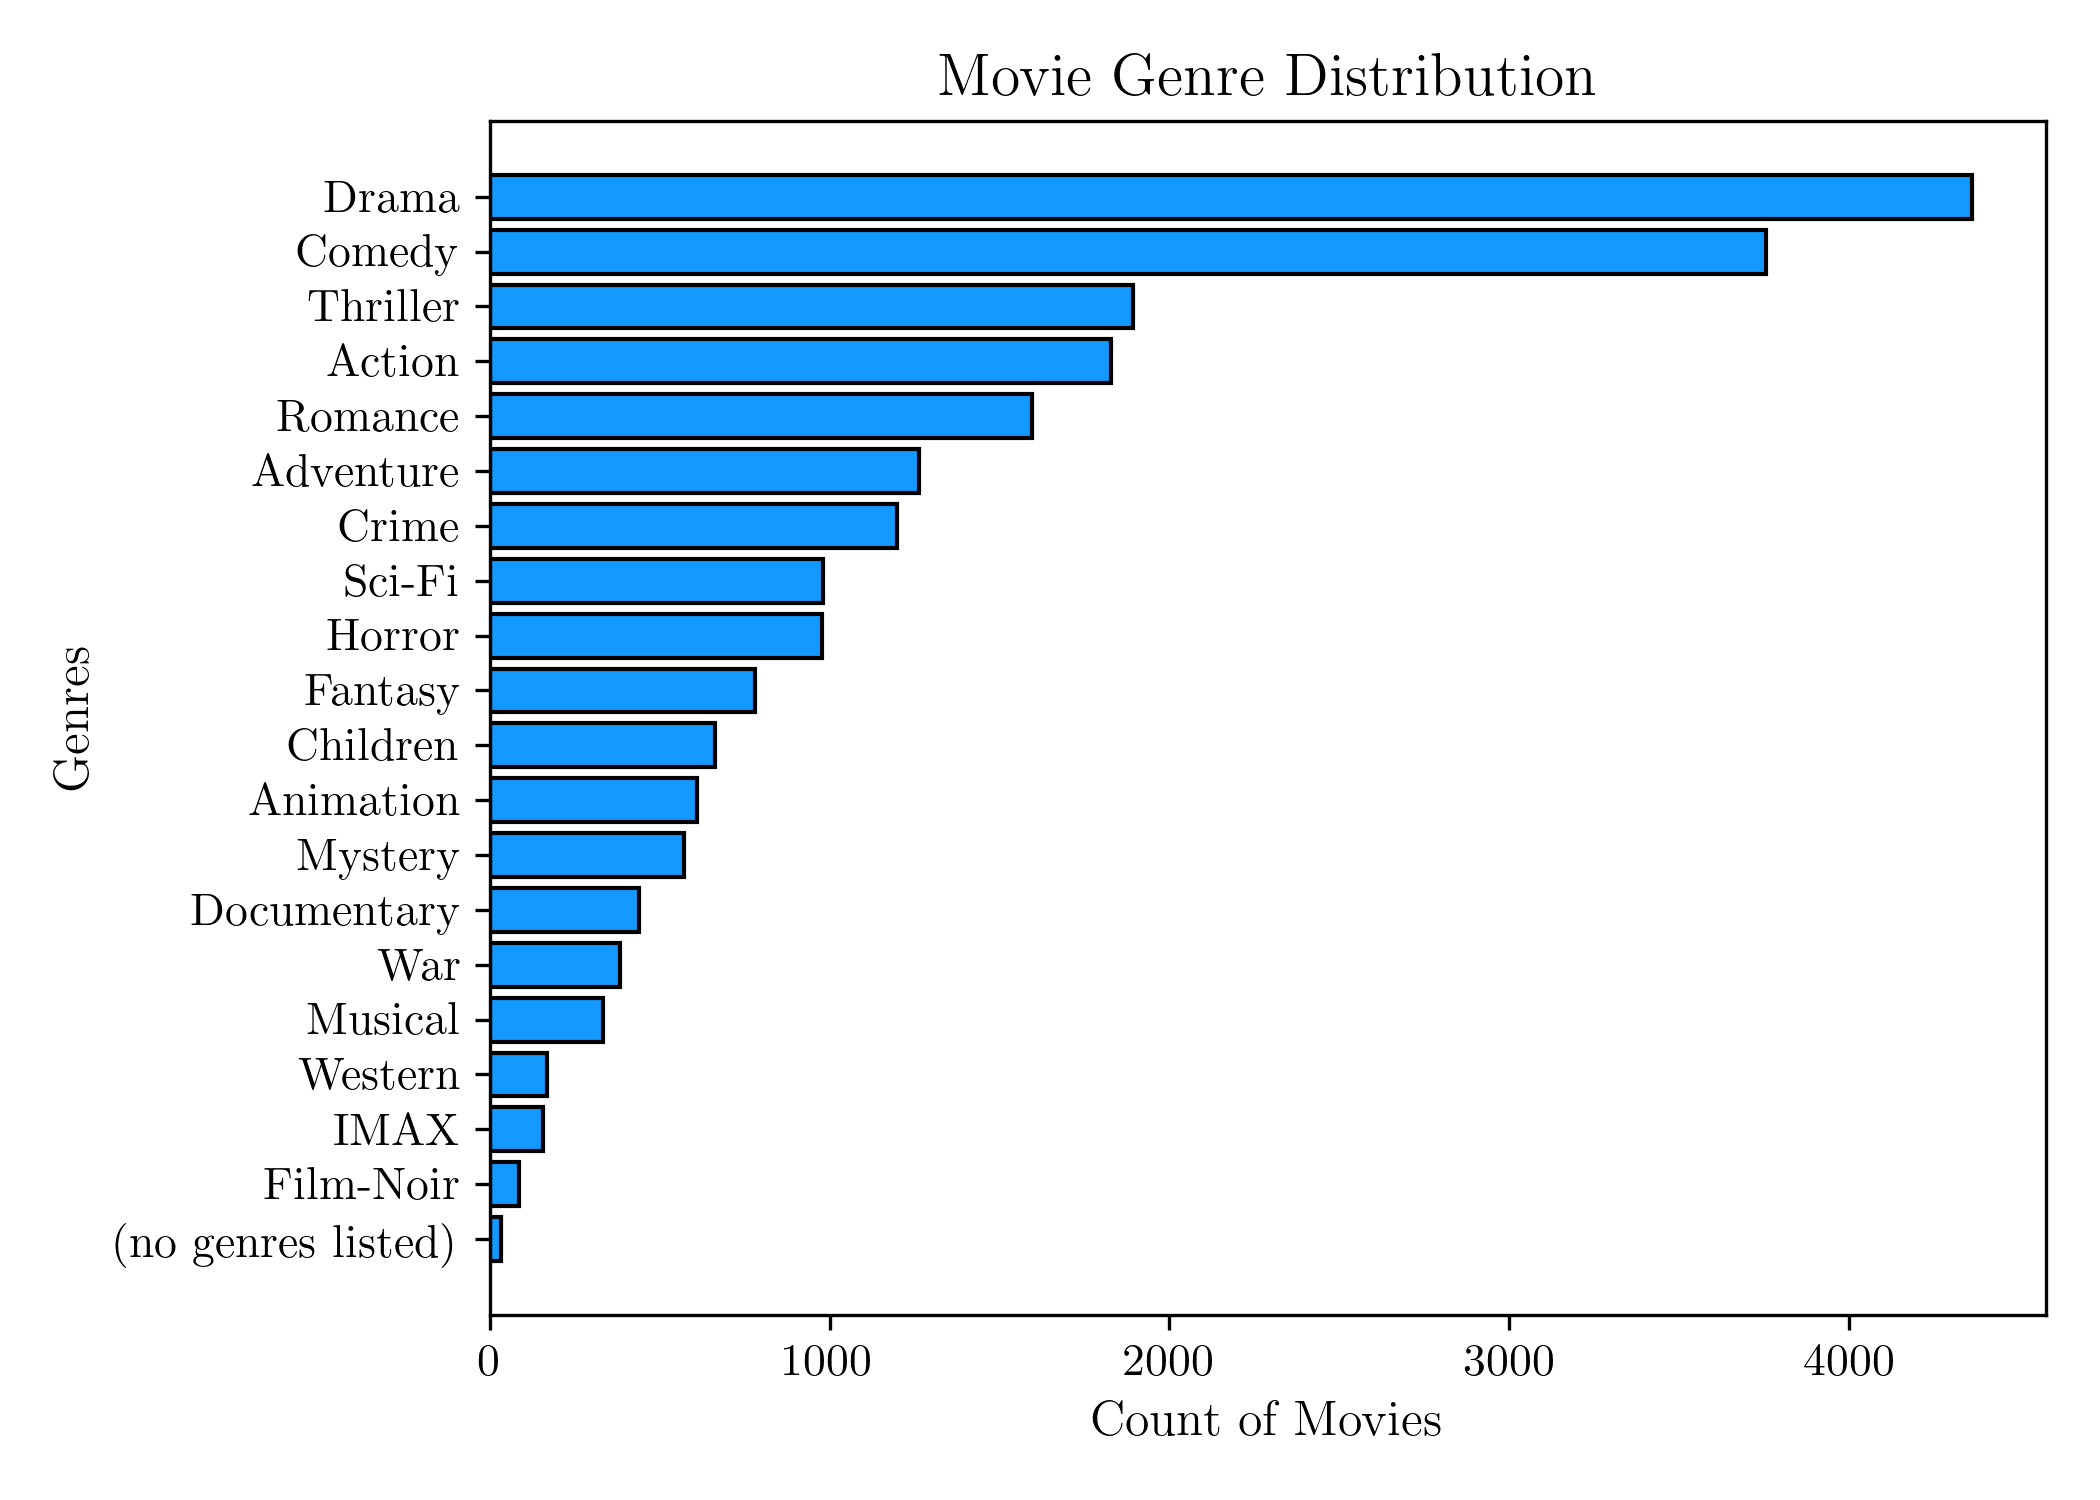
\includegraphics[width=1\linewidth]{assets/genre_distribution.png}
    \caption{Distribution of movies per movie genre.}
    \label{fig:genre_distribution}
\end{figure}

Despite the variety in genres, it's important to retain that generally movies are more complex than representing a single genre. In that sense, it is useful to assess the similarity between genres (using the cosine similarity index), as illustrated in Fig. \ref{fig:genre_similarity}. This helps understand how the task of recommending a movie can start to grow more complex as we add more and more detail to the dataset. In Table \ref{tab:genre_similarity} the five most related genres are shown.

\begin{figure}[H]
    \centering
    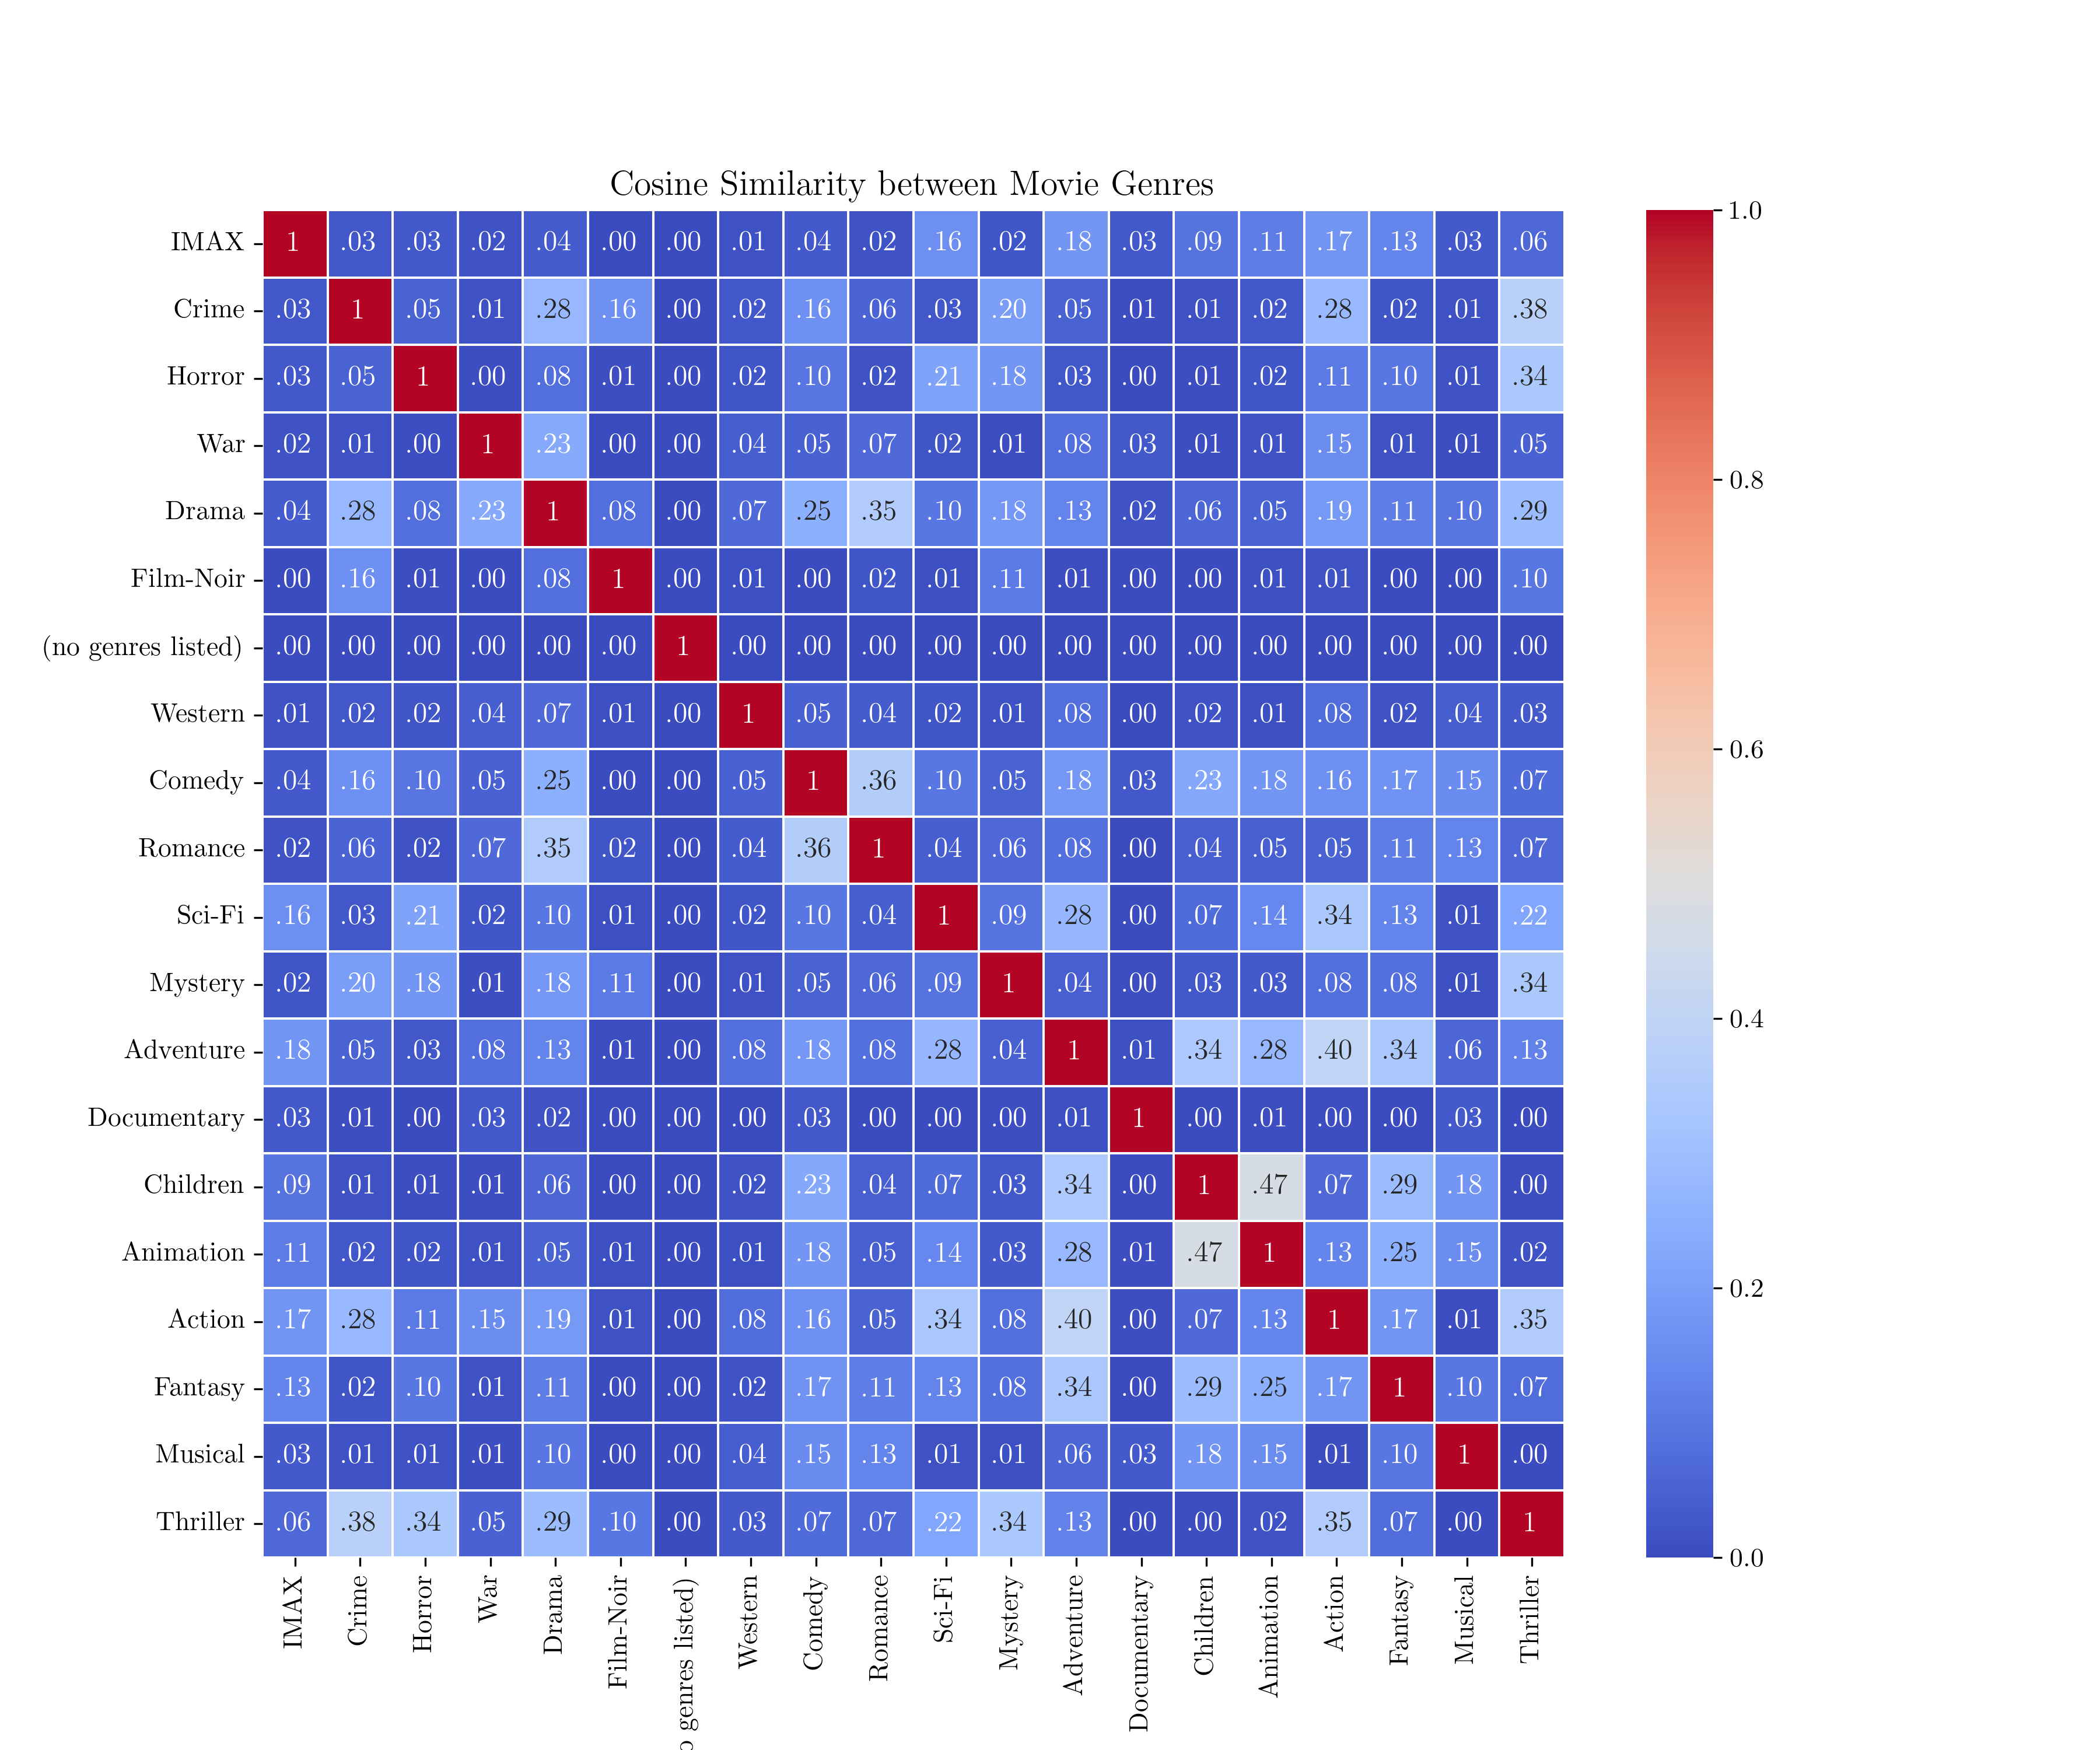
\includegraphics[width=1\linewidth]{assets/genre_similarity.png}
    \caption{Cosine similarity index between genres.}
    \label{fig:genre_similarity}
\end{figure}

\begin{table}[H]
\centering
\caption{The five most related genres per cosine similarity index.}
\label{tab:genre_similarity}
\begin{tabular}{llr}
\toprule
\textbf{Genre} & \textbf{Genre} & \textbf{Similarity index} \\
\midrule
Animation & Children & .47 \\ 
Action & Adventure & .40 \\
Crime & Thriller & .38 \\
Romance & Comedy & .36 \\
Romance & Drama & .35 \\
\bottomrule
\end{tabular}
\end{table} 

The dataset is relatively recent, with movies from the 2010's, going all the way back to the early 1900's, as per Fig. \ref{fig:year_distribution}. As expected, there are much less ratings for older movies, for two main reasons: older movies are less popular and there are less movies in general.

\begin{figure}[H]
    \centering
    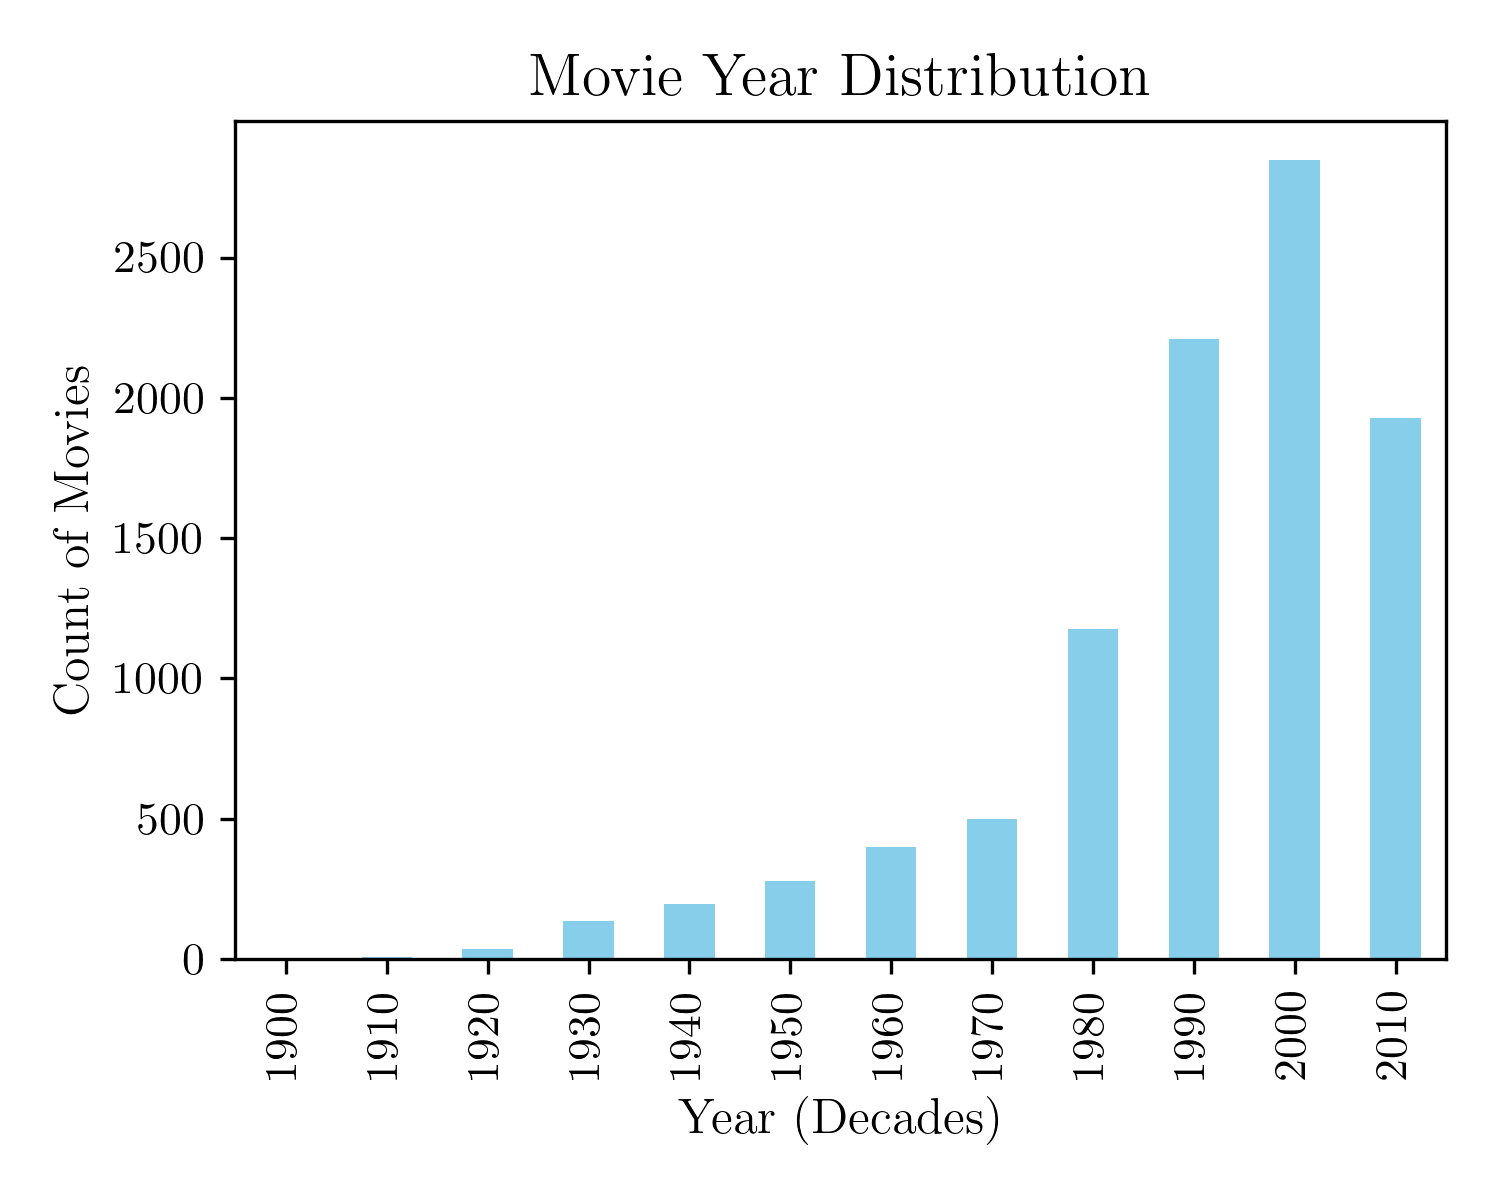
\includegraphics[width=1\linewidth]{assets/year_distribution.png}
    \caption{Distribution of movies per year.}
    \label{fig:year_distribution}
\end{figure}

As expected, both distributions from Fig. \ref{fig:distribution_moviesratings} and \ref{fig:distribution_userratings} are positively skewed as mentioned before. In general there are more people rating a small amount of movies, and the number of movies with higher counts of ratings tends to decrease rapidly (as there are very few, very popular movies).

This type of distribution is commonly found across recommender systems, and represents well the challenges posed to these algorithms: sparsity, whereas most of the matrix is empty (98.3 \% of missing values); bias, popular movies tend to dominate the analysis; and the long tail represents the challenge to make recommendations based on the large number of movies (or users) with very few ratings (or that rated few movies).

\begin{figure}[H]
    \centering
    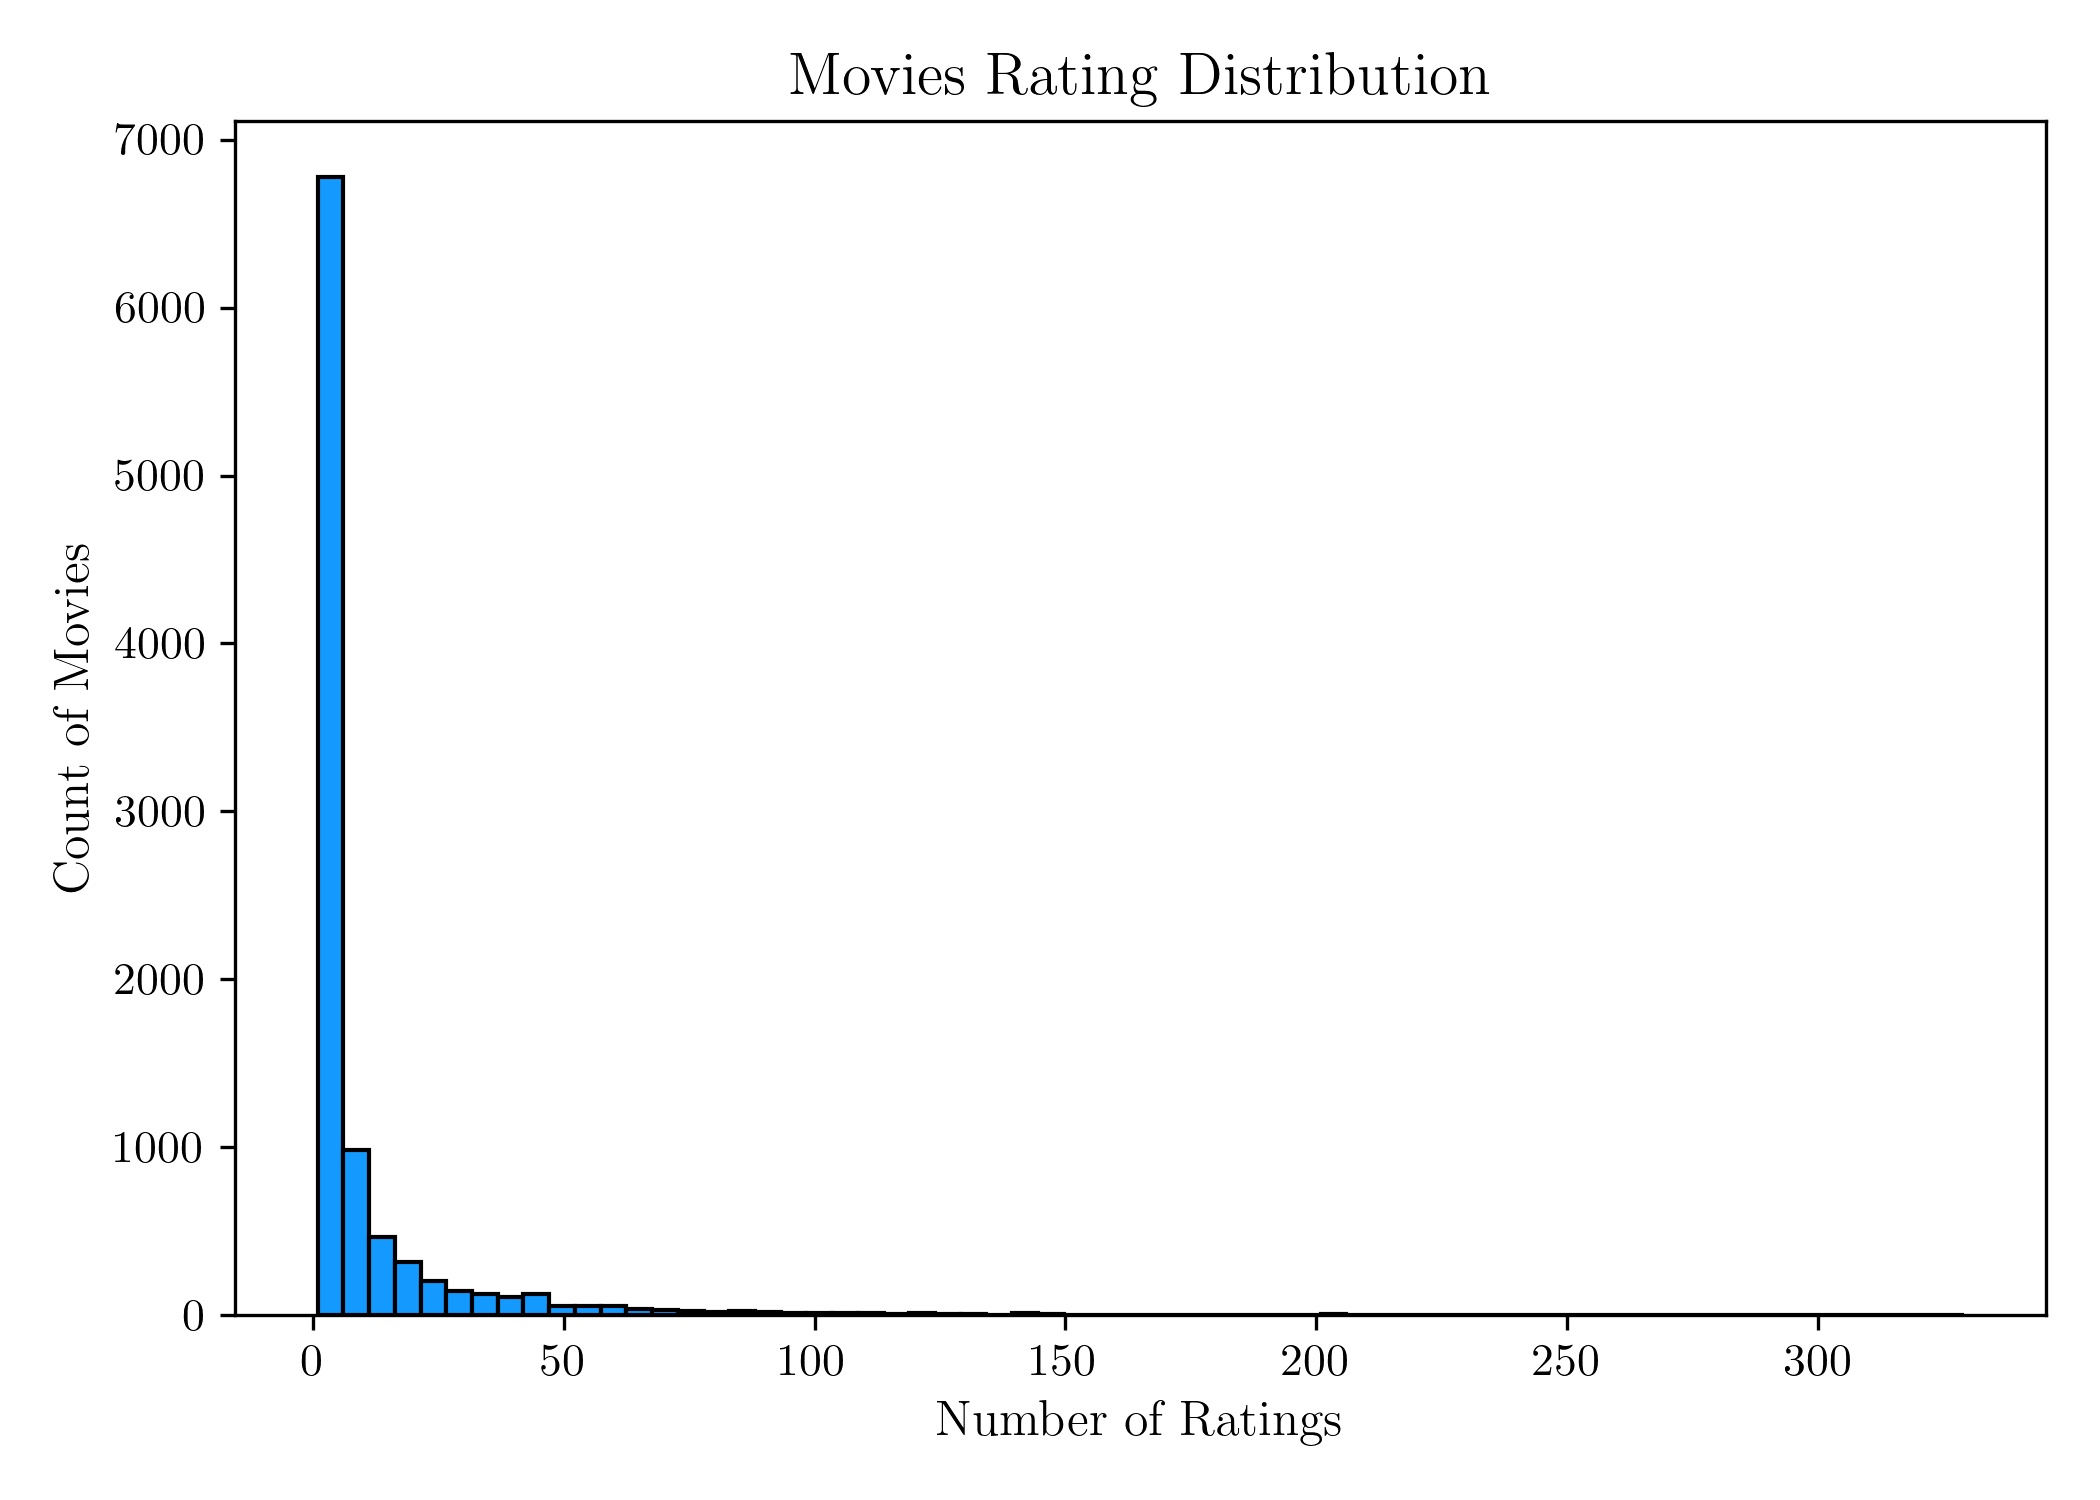
\includegraphics[width=1\linewidth]{assets/distribution_moviesratings.png}
    \caption{Distribution of the number of movies and the amount of ratings. The first bin correspond to 1 movie rated.}    \label{fig:distribution_moviesratings}
\end{figure}

To finalize, it is important to mention (again) that the minimum number of ratings per user is 20, and the maximum is 2698. The minimum rating per movie is 1, and the maximum is 329 ratings. The most rated movies (and not so coincidentally) the highest rated movies were:
\begin{itemize}
    \item Forrest Gump (1994) - 329 ratings
    \item Pulp Fiction (1994) - 317 ratings
    \item The Shawshank Redemption (1994) - 307 ratings
\end{itemize}


\begin{figure}[H]
    \centering
    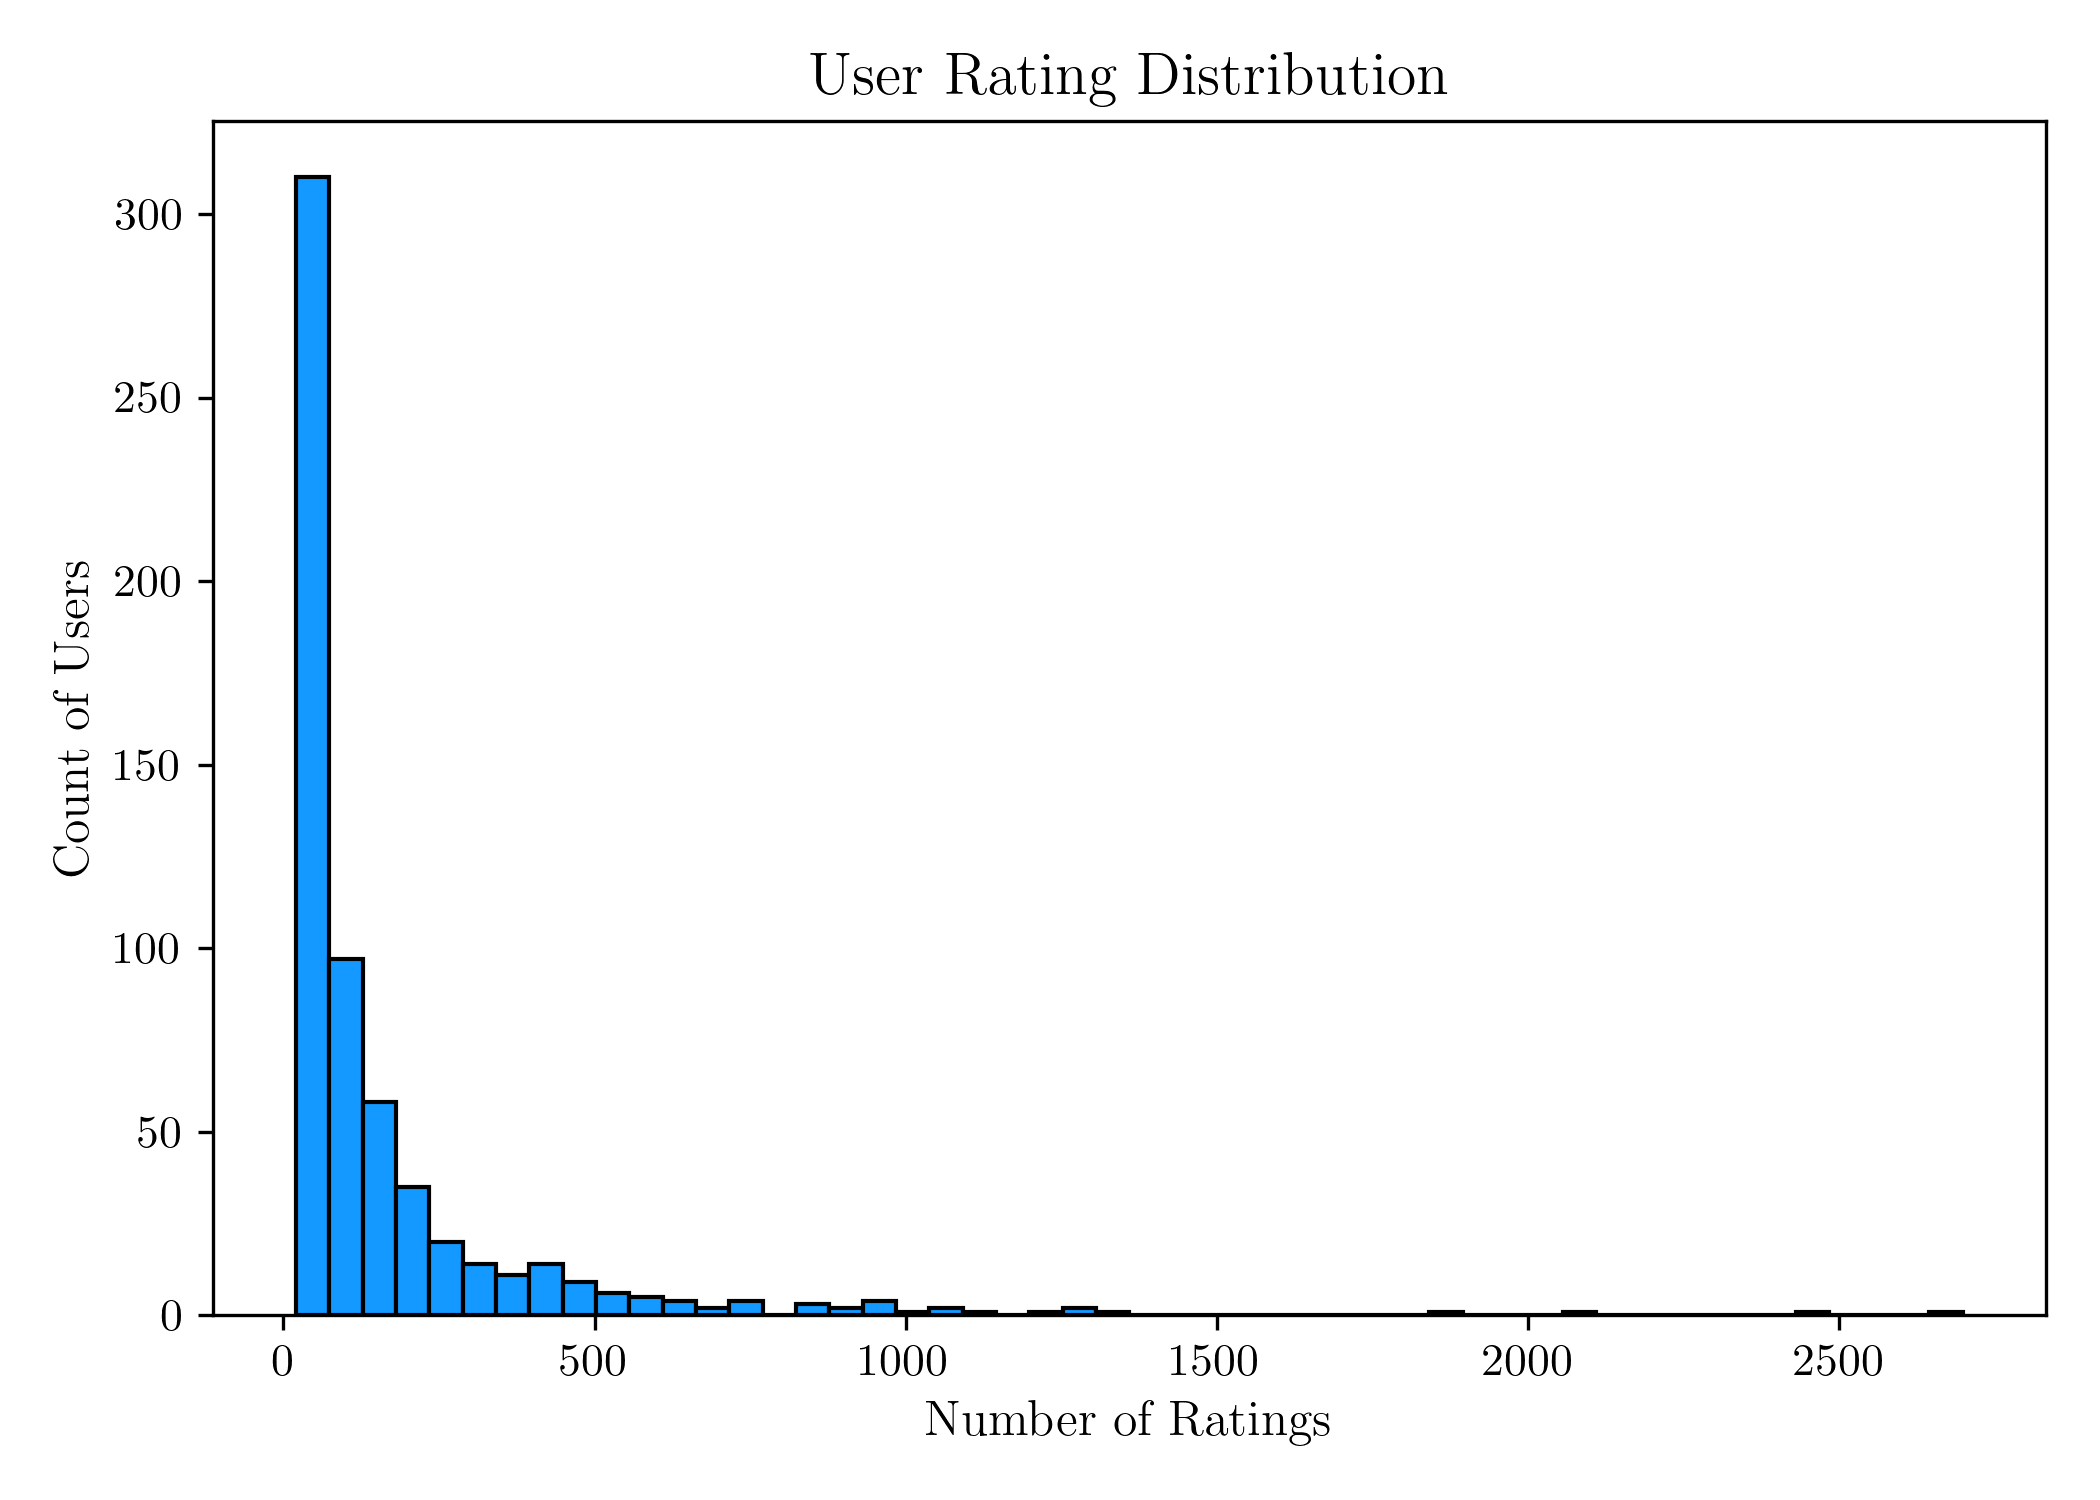
\includegraphics[width=1\linewidth]{assets/distribution_userratings.png}
    \caption{Distribution of the number of users and the amount of ratings. The first bin correspond to 20 movies rated.}    \label{fig:distribution_userratings}
\end{figure}

\subsection{MEDIDAS DE ERRO OU AVALIACAO}




\section{Classification Models}

The three models here presented are first and foremost linear regression problems, where by fitting a model with the known data to the users and the movies, it will be possible to estimate the ratings of movies that have not been reviewed. In this sense, besides the model itself, it is necessary to fit two hyperparameters, the learning rate $\alpha$, and the cost parameter $\lambda$. 

The first model developed aims to fit both users (\textit{x} parameter) and movies ($\theta$ parameter) simultaneously, as depicted in the equation below.
\begin{multline}
\min_{x^{(1)}, \dots, x^{(n_m)}, \theta^{(1)}, \dots, \theta^{(n_u)}} 
\frac{1}{2} \sum_{(i, j) : r(i, j) = 1} \left( (\theta^{(j)})^T x^{(i)} - y^{(i,j)} \right)^2 \\
+ \frac{\lambda}{2} \sum_{i=1}^{n_m} \sum_{k=1}^{n} \left( x_k^{(i)} \right)^2 + \frac{\lambda}{2} \sum_{j=1}^{n_u} \sum_{k=1}^{n} \left( \theta_k^{(j)} \right)^2
\end{multline}


The second model fits only the users parameter, given that it accounts for the movies parameters by using the movie genres.
\begin{align}
\min_{\theta^{(1)}, \dots, \theta^{(n_u)}} 
&\frac{1}{2} \sum_{j=1}^{n_u} \sum_{i : r(i, j) = 1} \left( (\theta^{(j)})^T x^{(i)} - y^{(i,j)} \right)^2 \notag \\
&+ \frac{\lambda}{2} \sum_{j=1}^{n_u} \sum_{k=1}^{n} \left( \theta_k^{(j)} \right)^2
\end{align}

\subsection{Model01 - LR}

Different ranges of $\alpha$ (between 0.0001 and 0.002) and $\lambda$ (between 0 and 100) were given to the model to be fit by usin 8 cross-validation in the training dataset. This allowed to progressively lower RMSE, throughout 500 iterations.

The best hyperparameters for Model01 were $\lambda = 6$ and $\alpha = 0.0005$, with an average RMSE from 8-CV of 1.25622.

\begin{figure}[H]
    \centering
    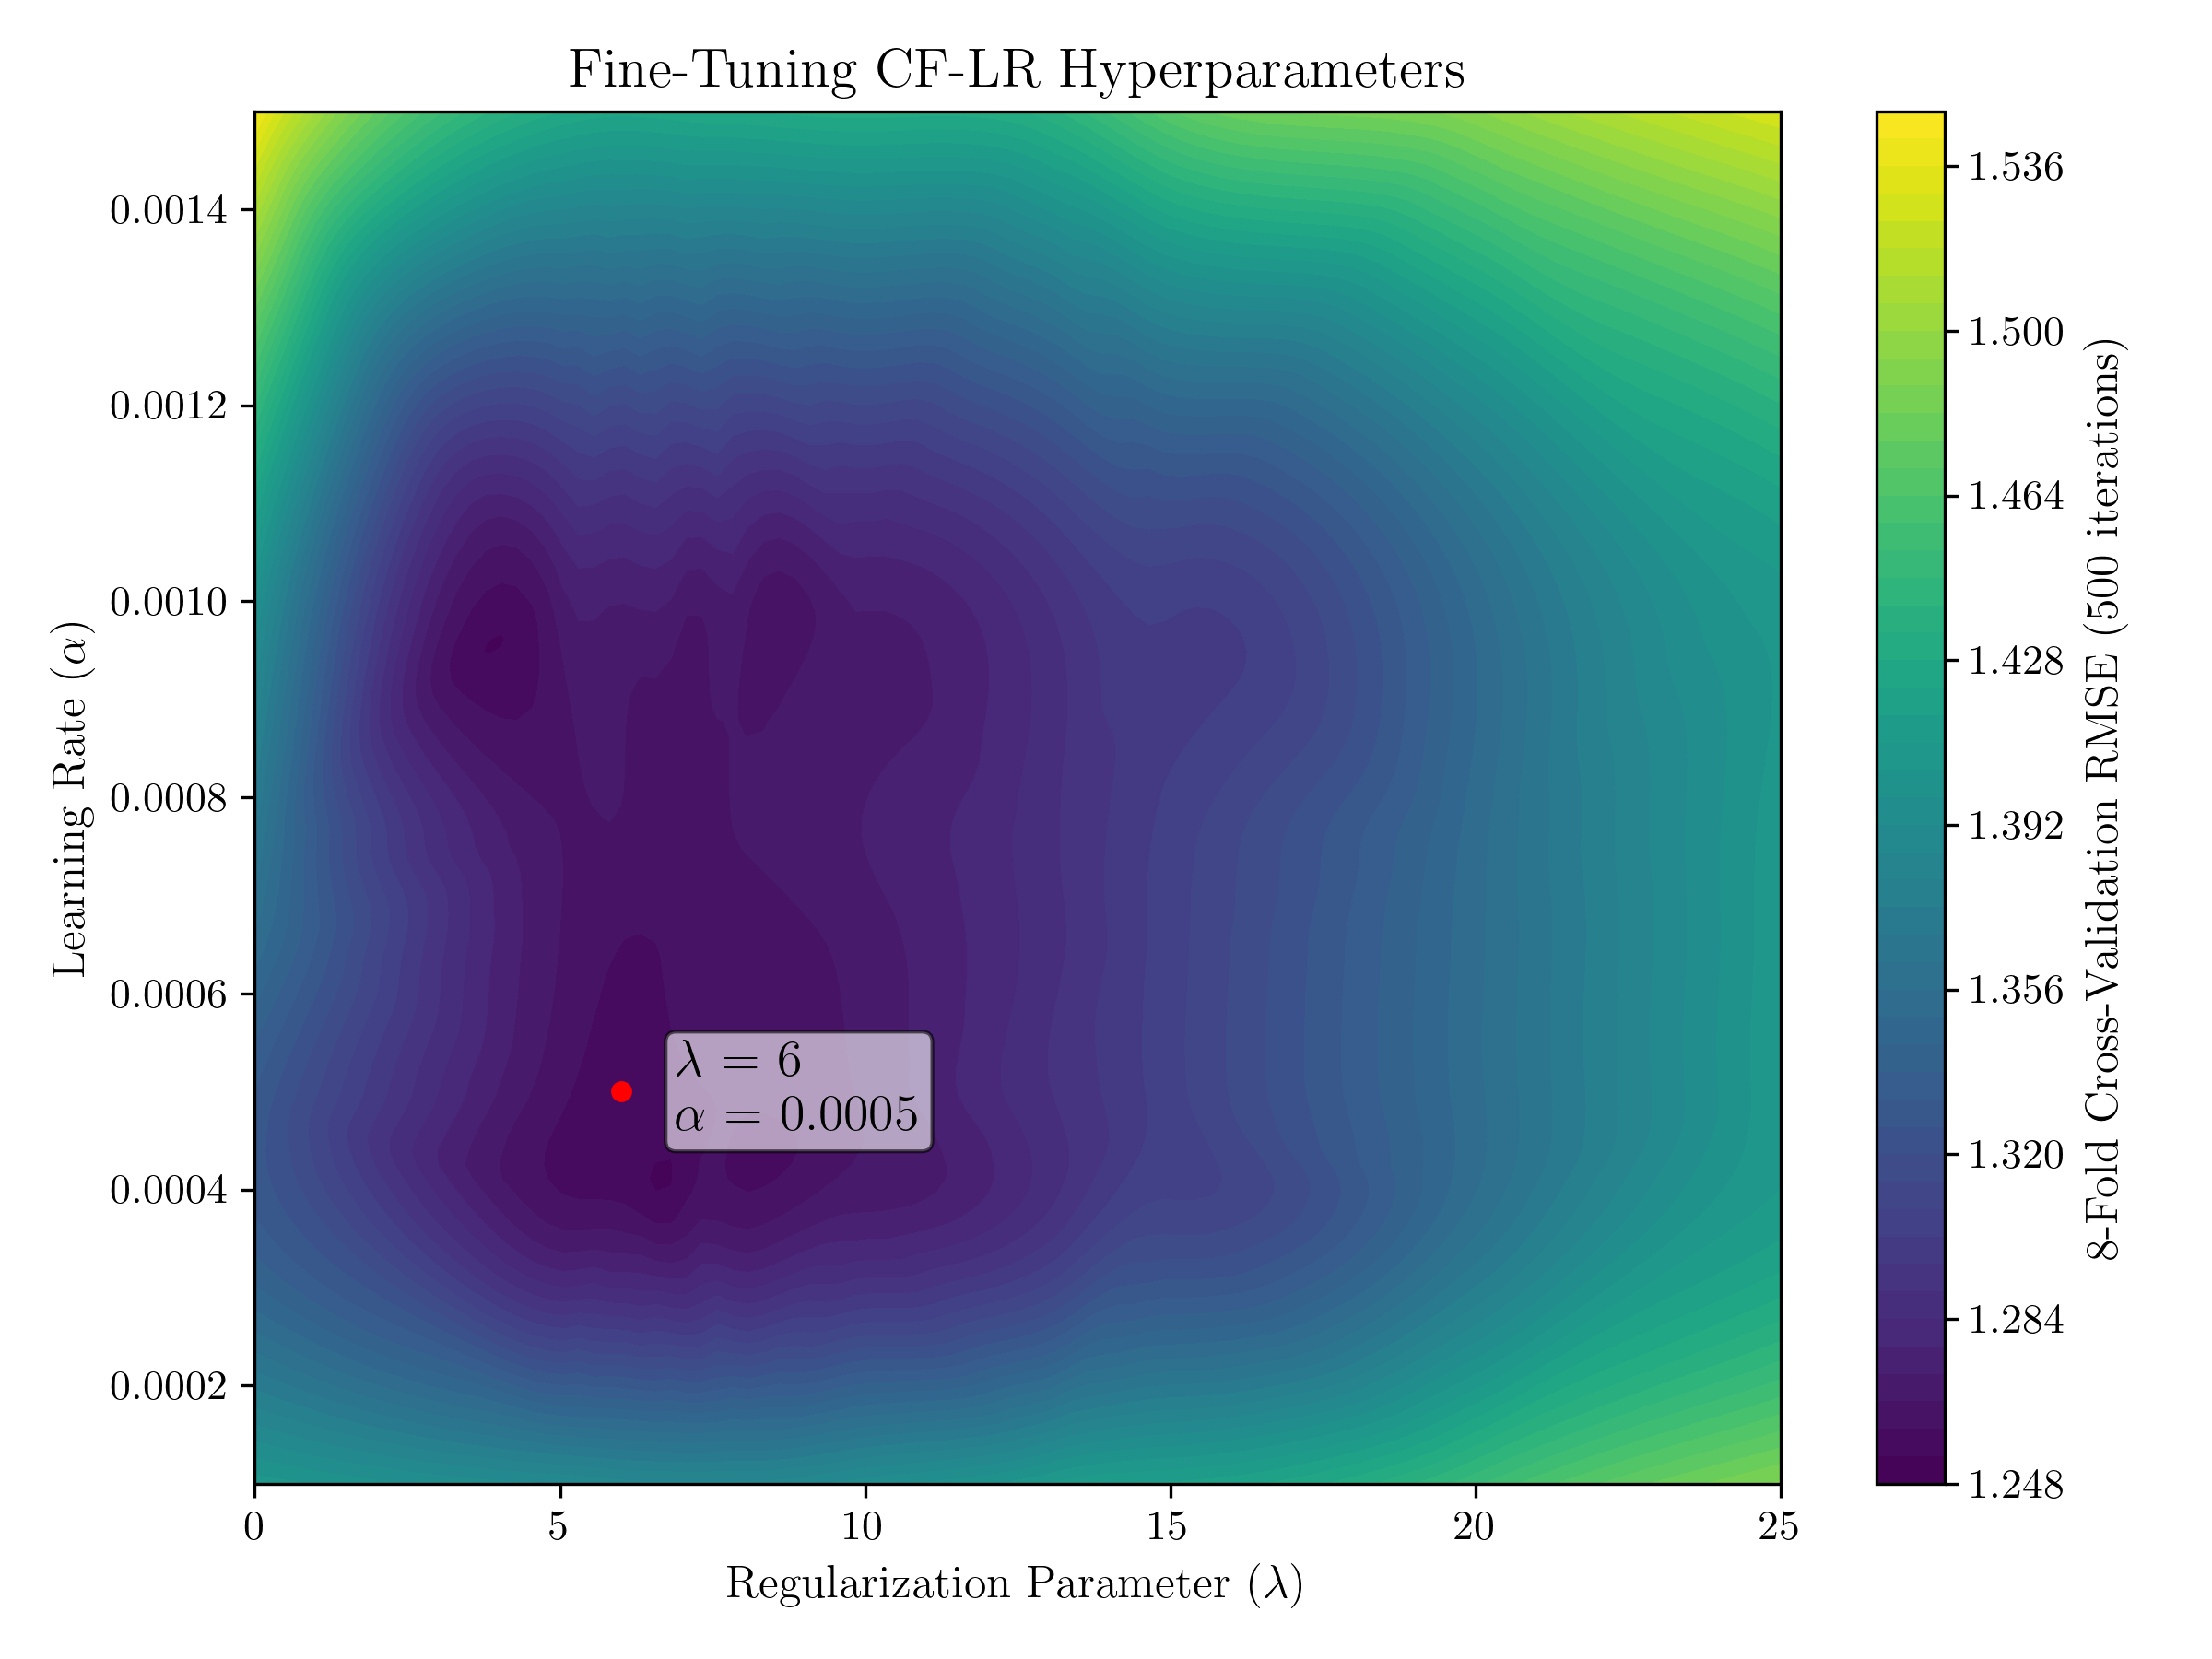
\includegraphics[width=1\linewidth]{assets/model01_hyperparametres.png}
    \caption{Learning rate ($\alpha$) and regularization parameter ($\lambda$) fitting.}
    \label{fig:model01_hyperparametres}
\end{figure}

Once the optimal hyperparameters were defined, the learning curve was estimated from the 8 CV on the training dataset, to assess the validity of the model and that it is not overfit.

\begin{figure}[H]
    \centering
    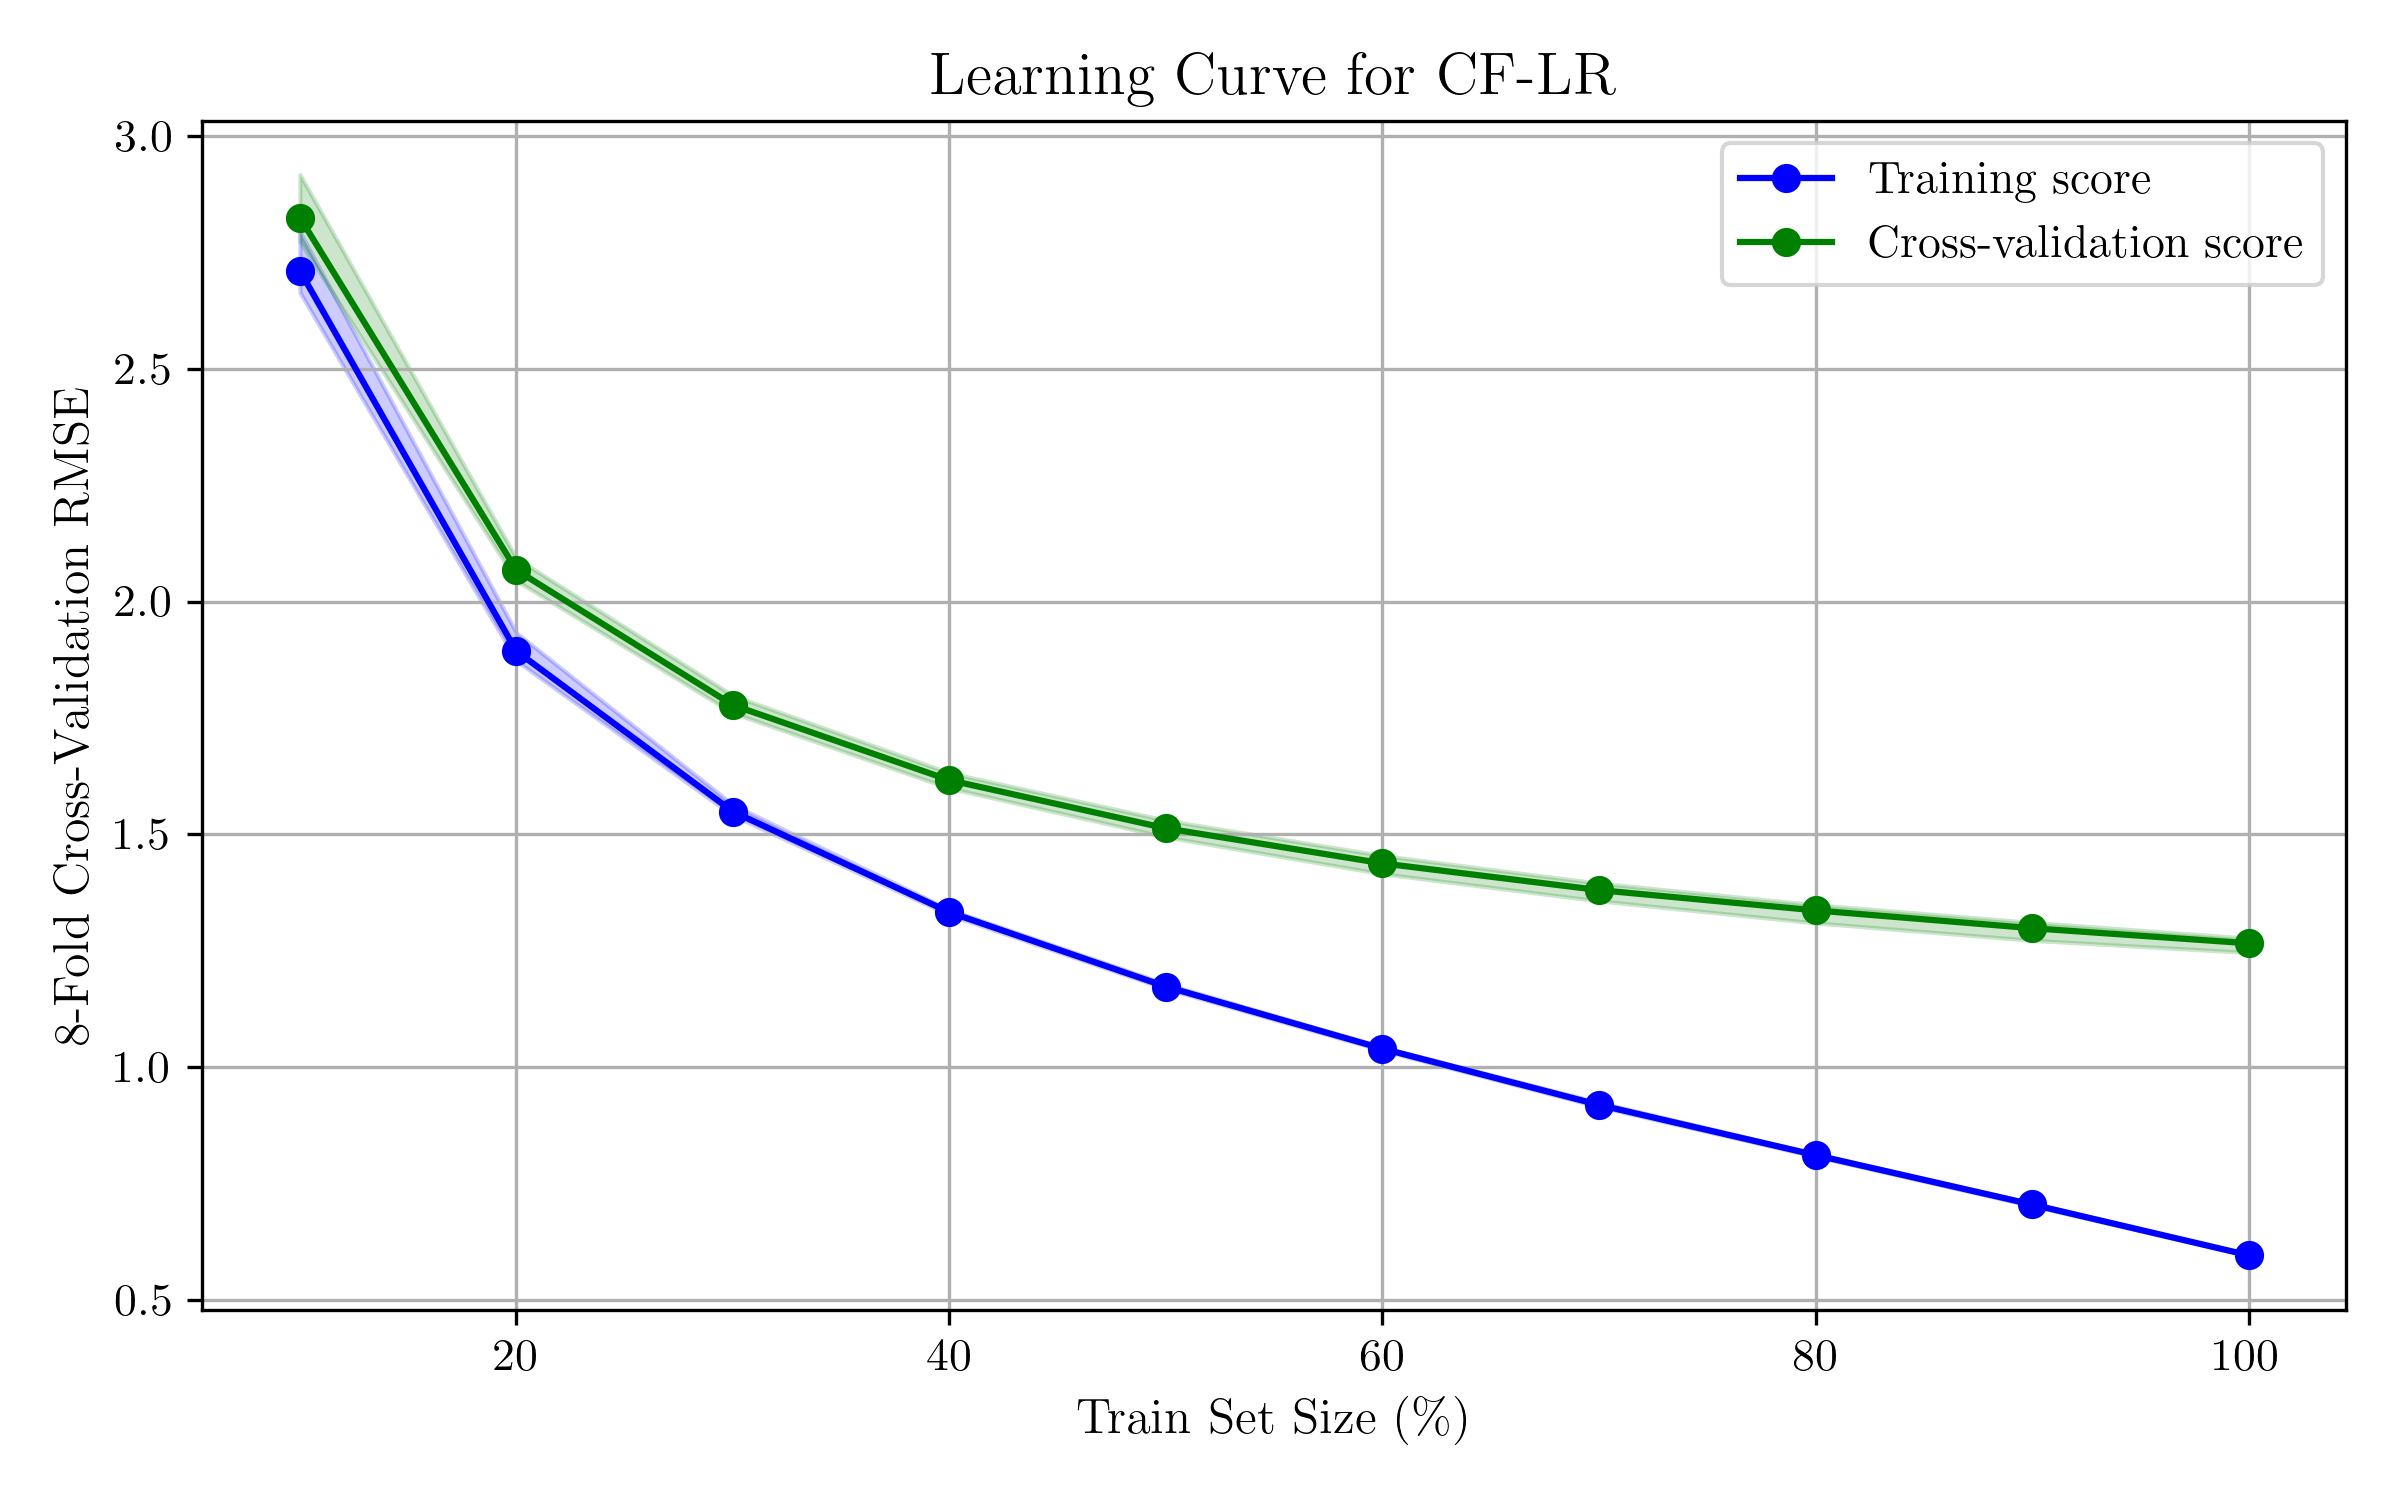
\includegraphics[width=1\linewidth]{assets/model01_learning_curve.png}
    \caption{Learning curve, RMSE progression throughout the training dataset.}
    \label{fig:model01_cost_function}
\end{figure}

DIZER Q USAMOS 20 FEATURES PARA X E 20 PARA THETA PQ TEMOS 20 GENEROS DE FILMES E FOI DE FORMA EMPIRICA A ESCOLHA

tlvz haja um pouco d eoverffiting, visto que as retas comecam a divergir um pouco , e dps os resultados do rmse e q vao mostrar isso: DIZER Q PODEMOS TER UM POUCO DE OVERFFTING OQ SE PODE DEVER A ESTARMOS A OTIMZIAR 40 FEATURES, dizer aqui q podemos ter, dps da tabela do rmse, dizer q é possivel q tenhamos, pelo q tlvz fosse interessante otimizar o numero de features, num futuro trabalho OUUU dizer q nu futuro trabalho se pode exprimentar tbm outro tipo de regularizacao, usamos ridge, podiamos exprimentar lasso

dps foi entao aplicada a descida do gradiente? regressao linear? para obter a estimativa dos parametros x e theta (movies e users) do problema.

a figura seguinte mostra a funcao custo ao longo das iteracoes, revelanco a convergencia da mesma

\begin{figure}[H]
    \centering
    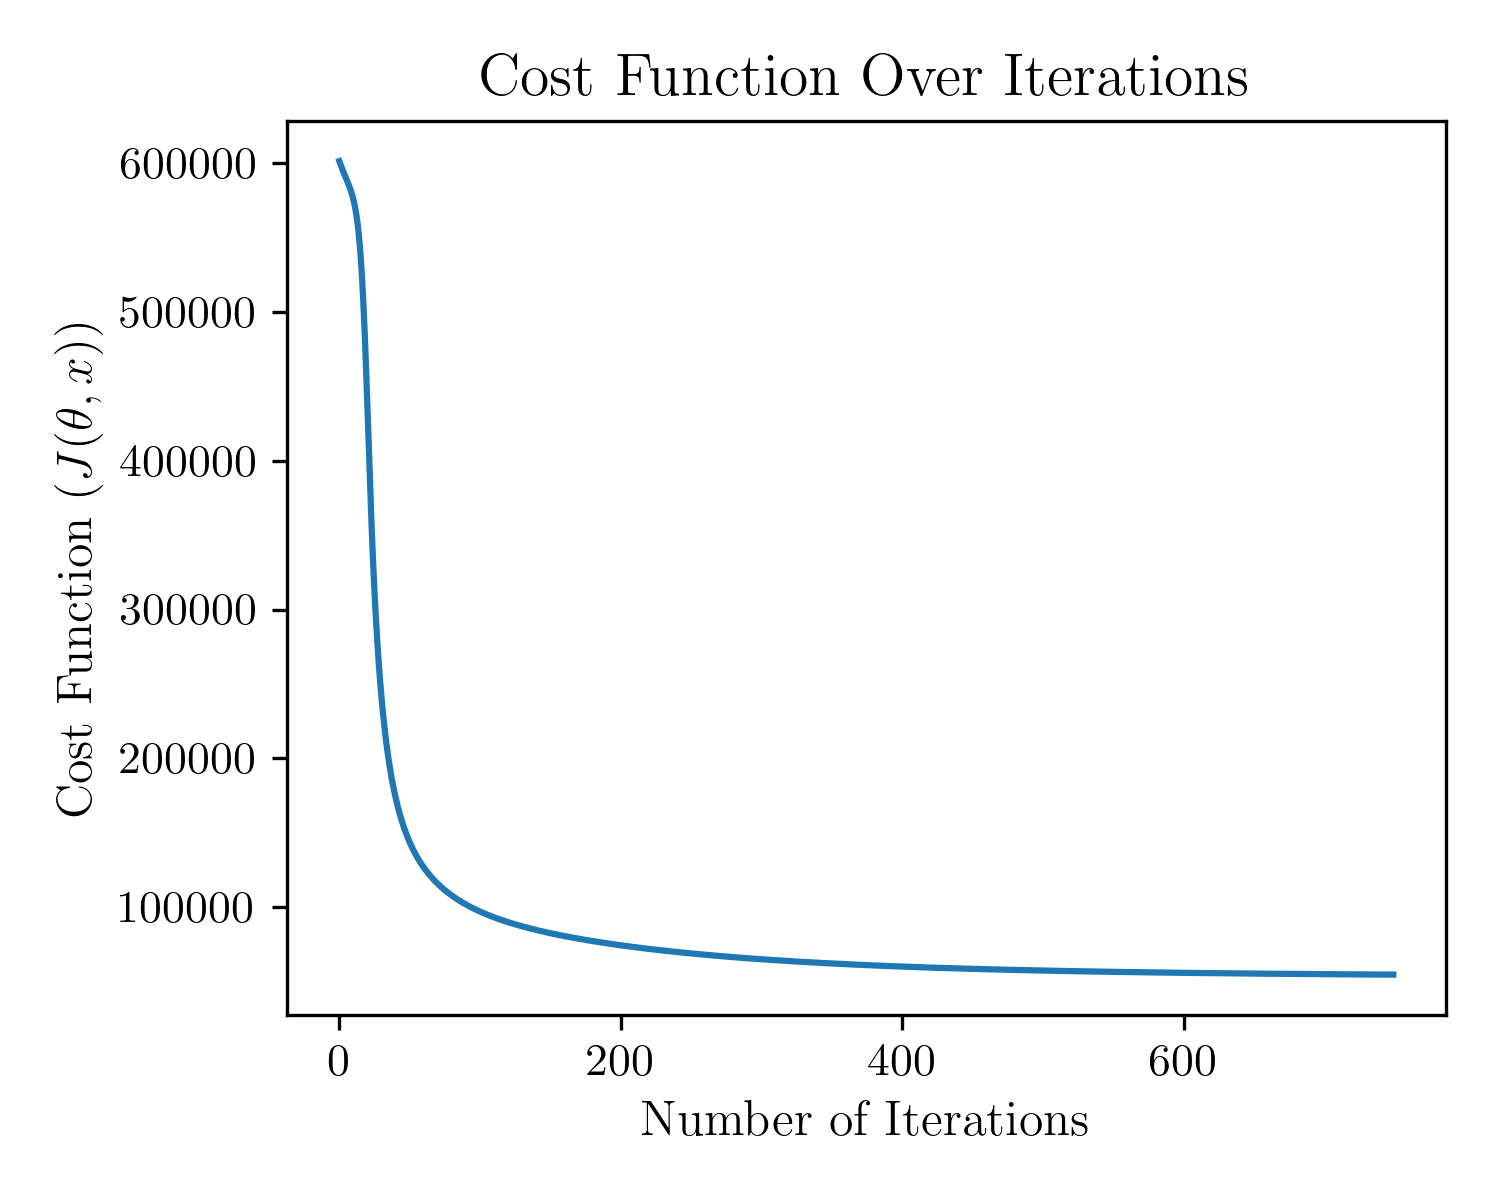
\includegraphics[width=1\linewidth]{assets/model01_cost_function.png}
    \caption{Cost function evolution with the number of iterations in the training set.}
    \label{fig:model01_cost_function}
\end{figure}

apos a estimativa dos ratings para todas as combinacoes de movies e users, compararam-se estas estimativas com as presentes na train e test data

\begin{table}[H]
\centering
\caption{CAPTIO CAPTION CAPTION}
\label{tab:model01_results}
\begin{tabular}{lccc}
\toprule
\textbf{Dataset} & \textbf{RMSE} & \textbf{MAE} & \textbf{Support} \\
\midrule
Train Set & 0.58842 & 0.44604 & 80668 \\
Test Set & 1.24037 & 0.90651 & 20168 \\
\bottomrule
\end{tabular}
\end{table}

\subsection{Model02 - LRC}

aqui é igual ao primeiro modelo mas ao inves de termos o x? (movies features) vamos ter os generos dos filmes, por exemplo se um filme é romance/drama é [0,0,....5,.5] tipo

ns q mesmos dados de treino e de teste de smp

neste caso temos o X q n precisa de otimizacao, pq é usado os generos dos filmes como features dos movies, content based, ent so vamos otimizar o theta (20 features dos users)

entre alpha 0.007 e 0.0005 e lambda 10 e 0, foram otimizados os hyperparametros, como se pode ver na figura uma parte desse intervalo, para melhor visuazalicao da otimizacao, tendo sido esta com minimizacao do rmse e 8cv nos dados de treino

\begin{figure}[H]
    \centering
    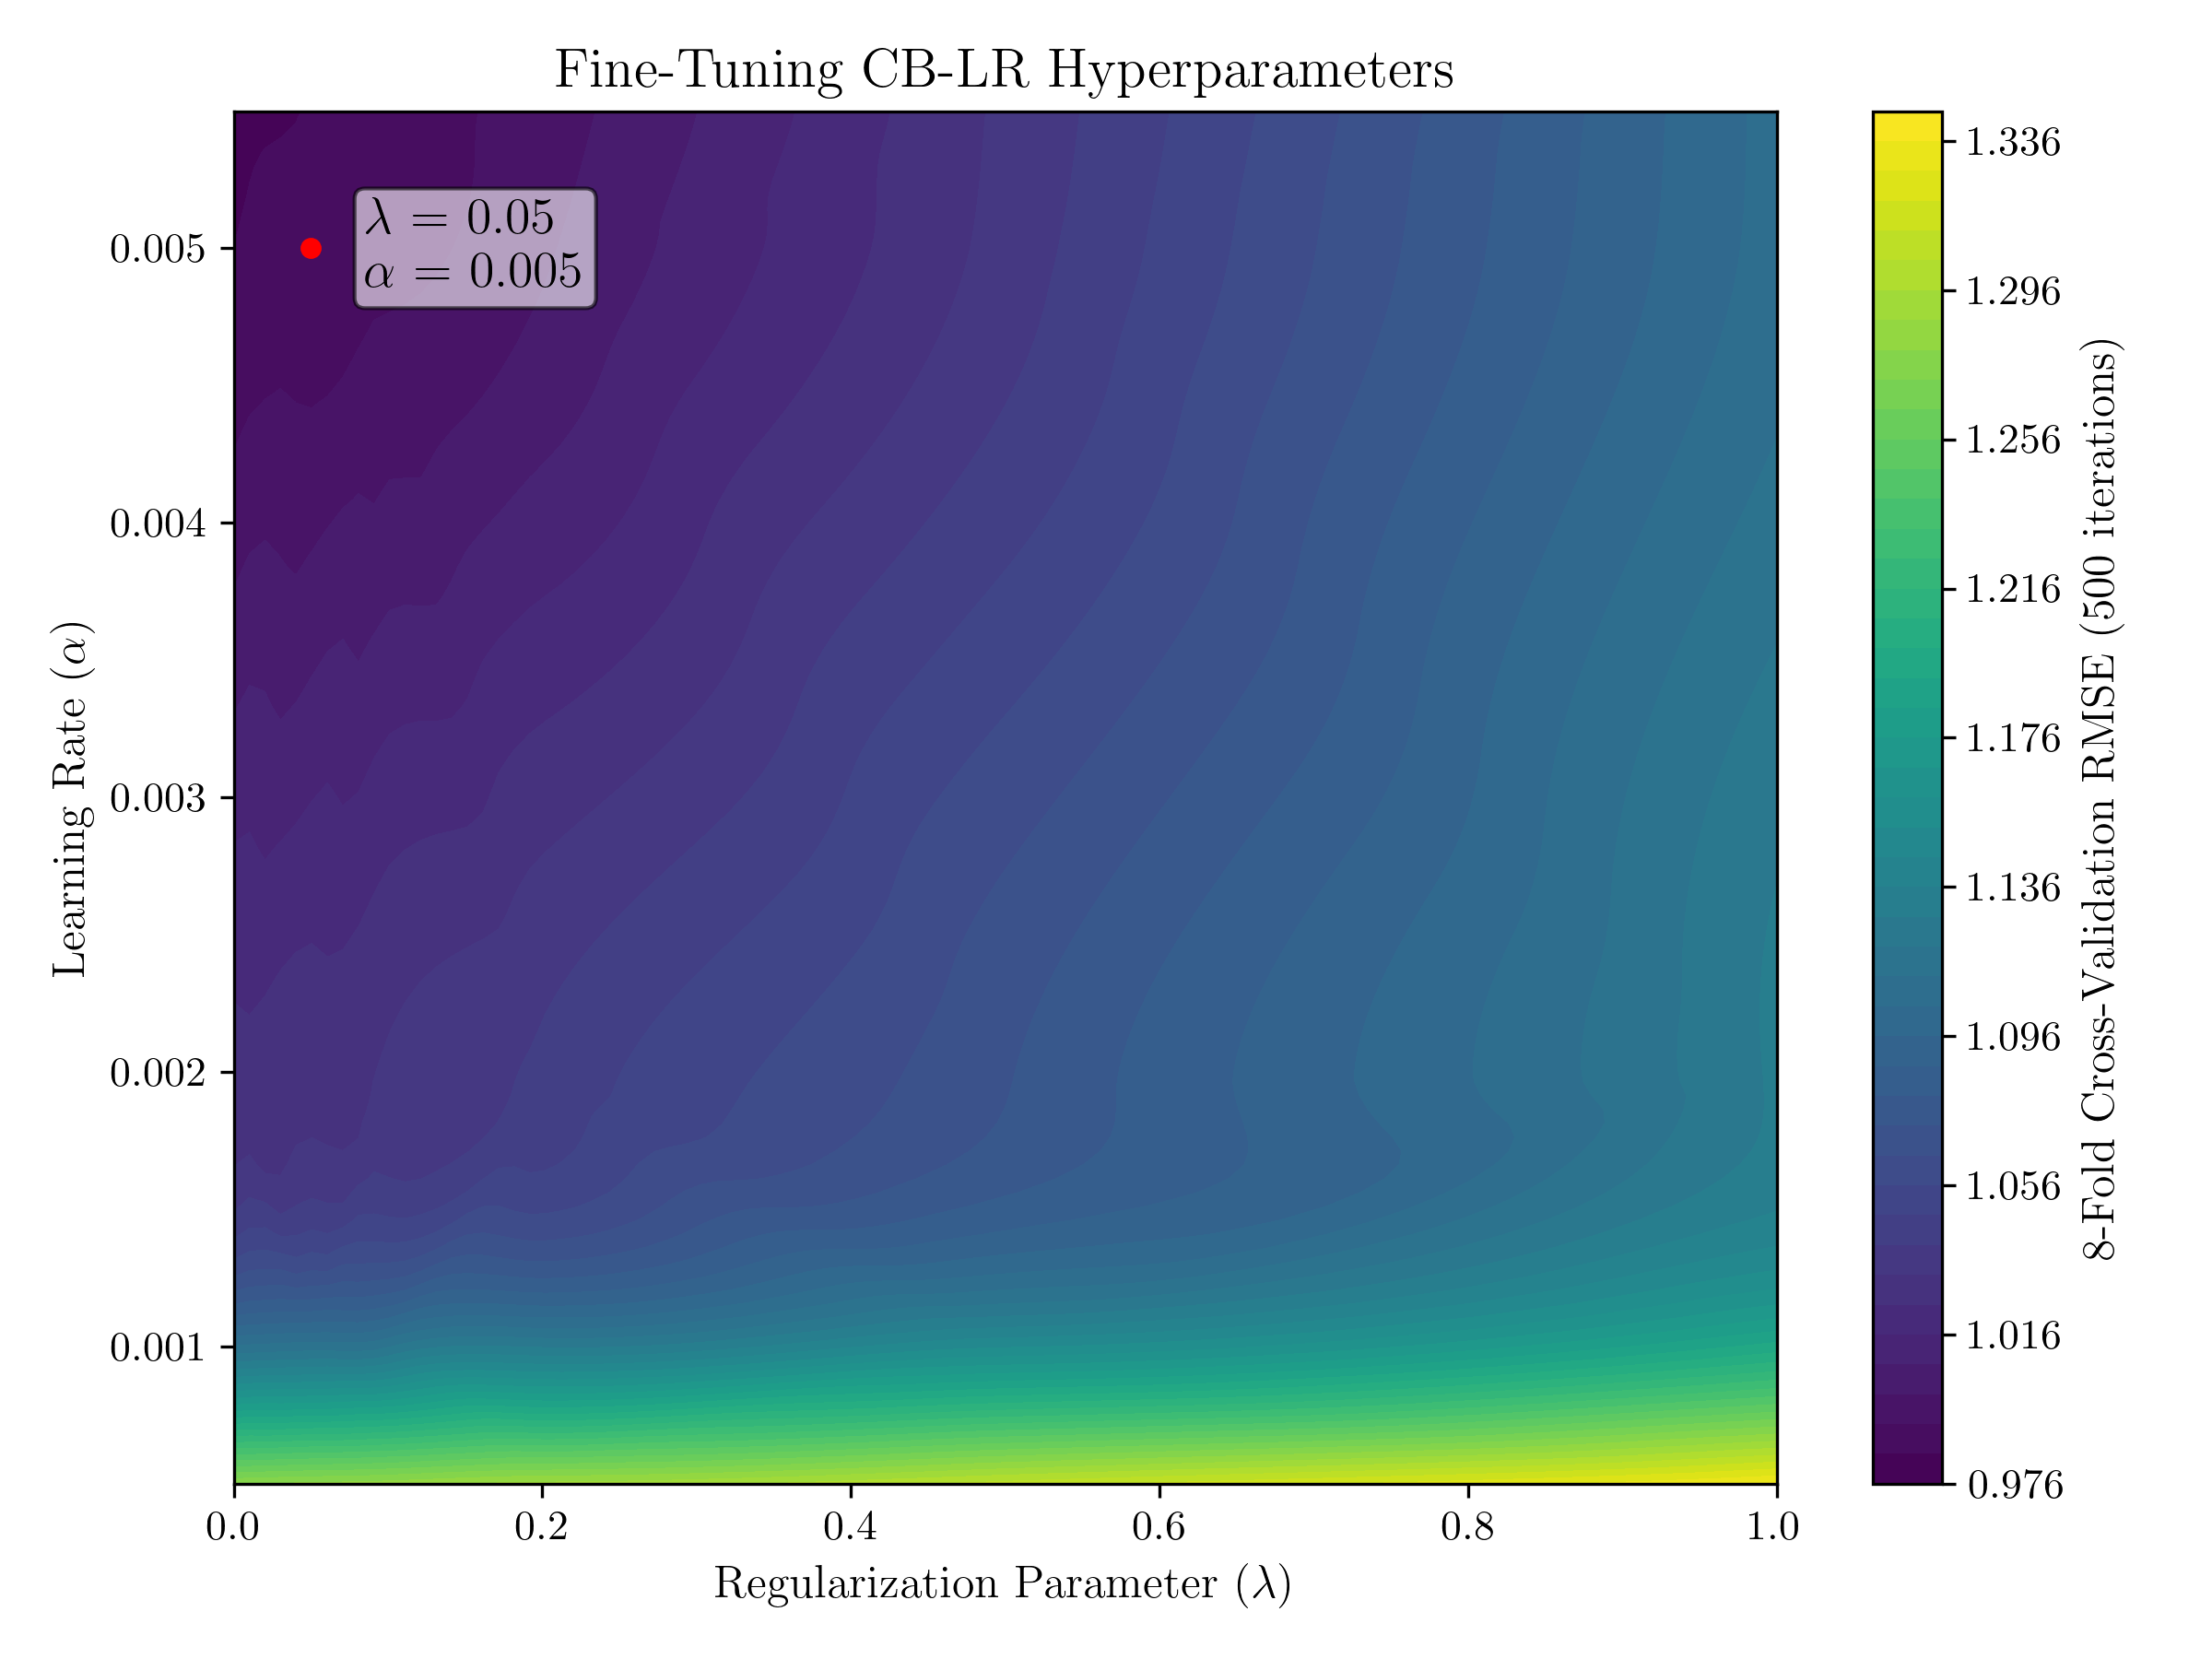
\includegraphics[width=1\linewidth]{assets/model02_hyperparemeterstunning.png}
    \caption{CAPTIO CAPTION CAPTION}
    \label{fig:model02_hyperparemeterstunning}
\end{figure}

The best hyperparameters are: (0.05, 0.005) with 8cv RMSE: 0.98617


de movo a verificar a validade do modelo, temos a learning curve, a ver se n ha overfiting

\begin{figure}[H]
    \centering
    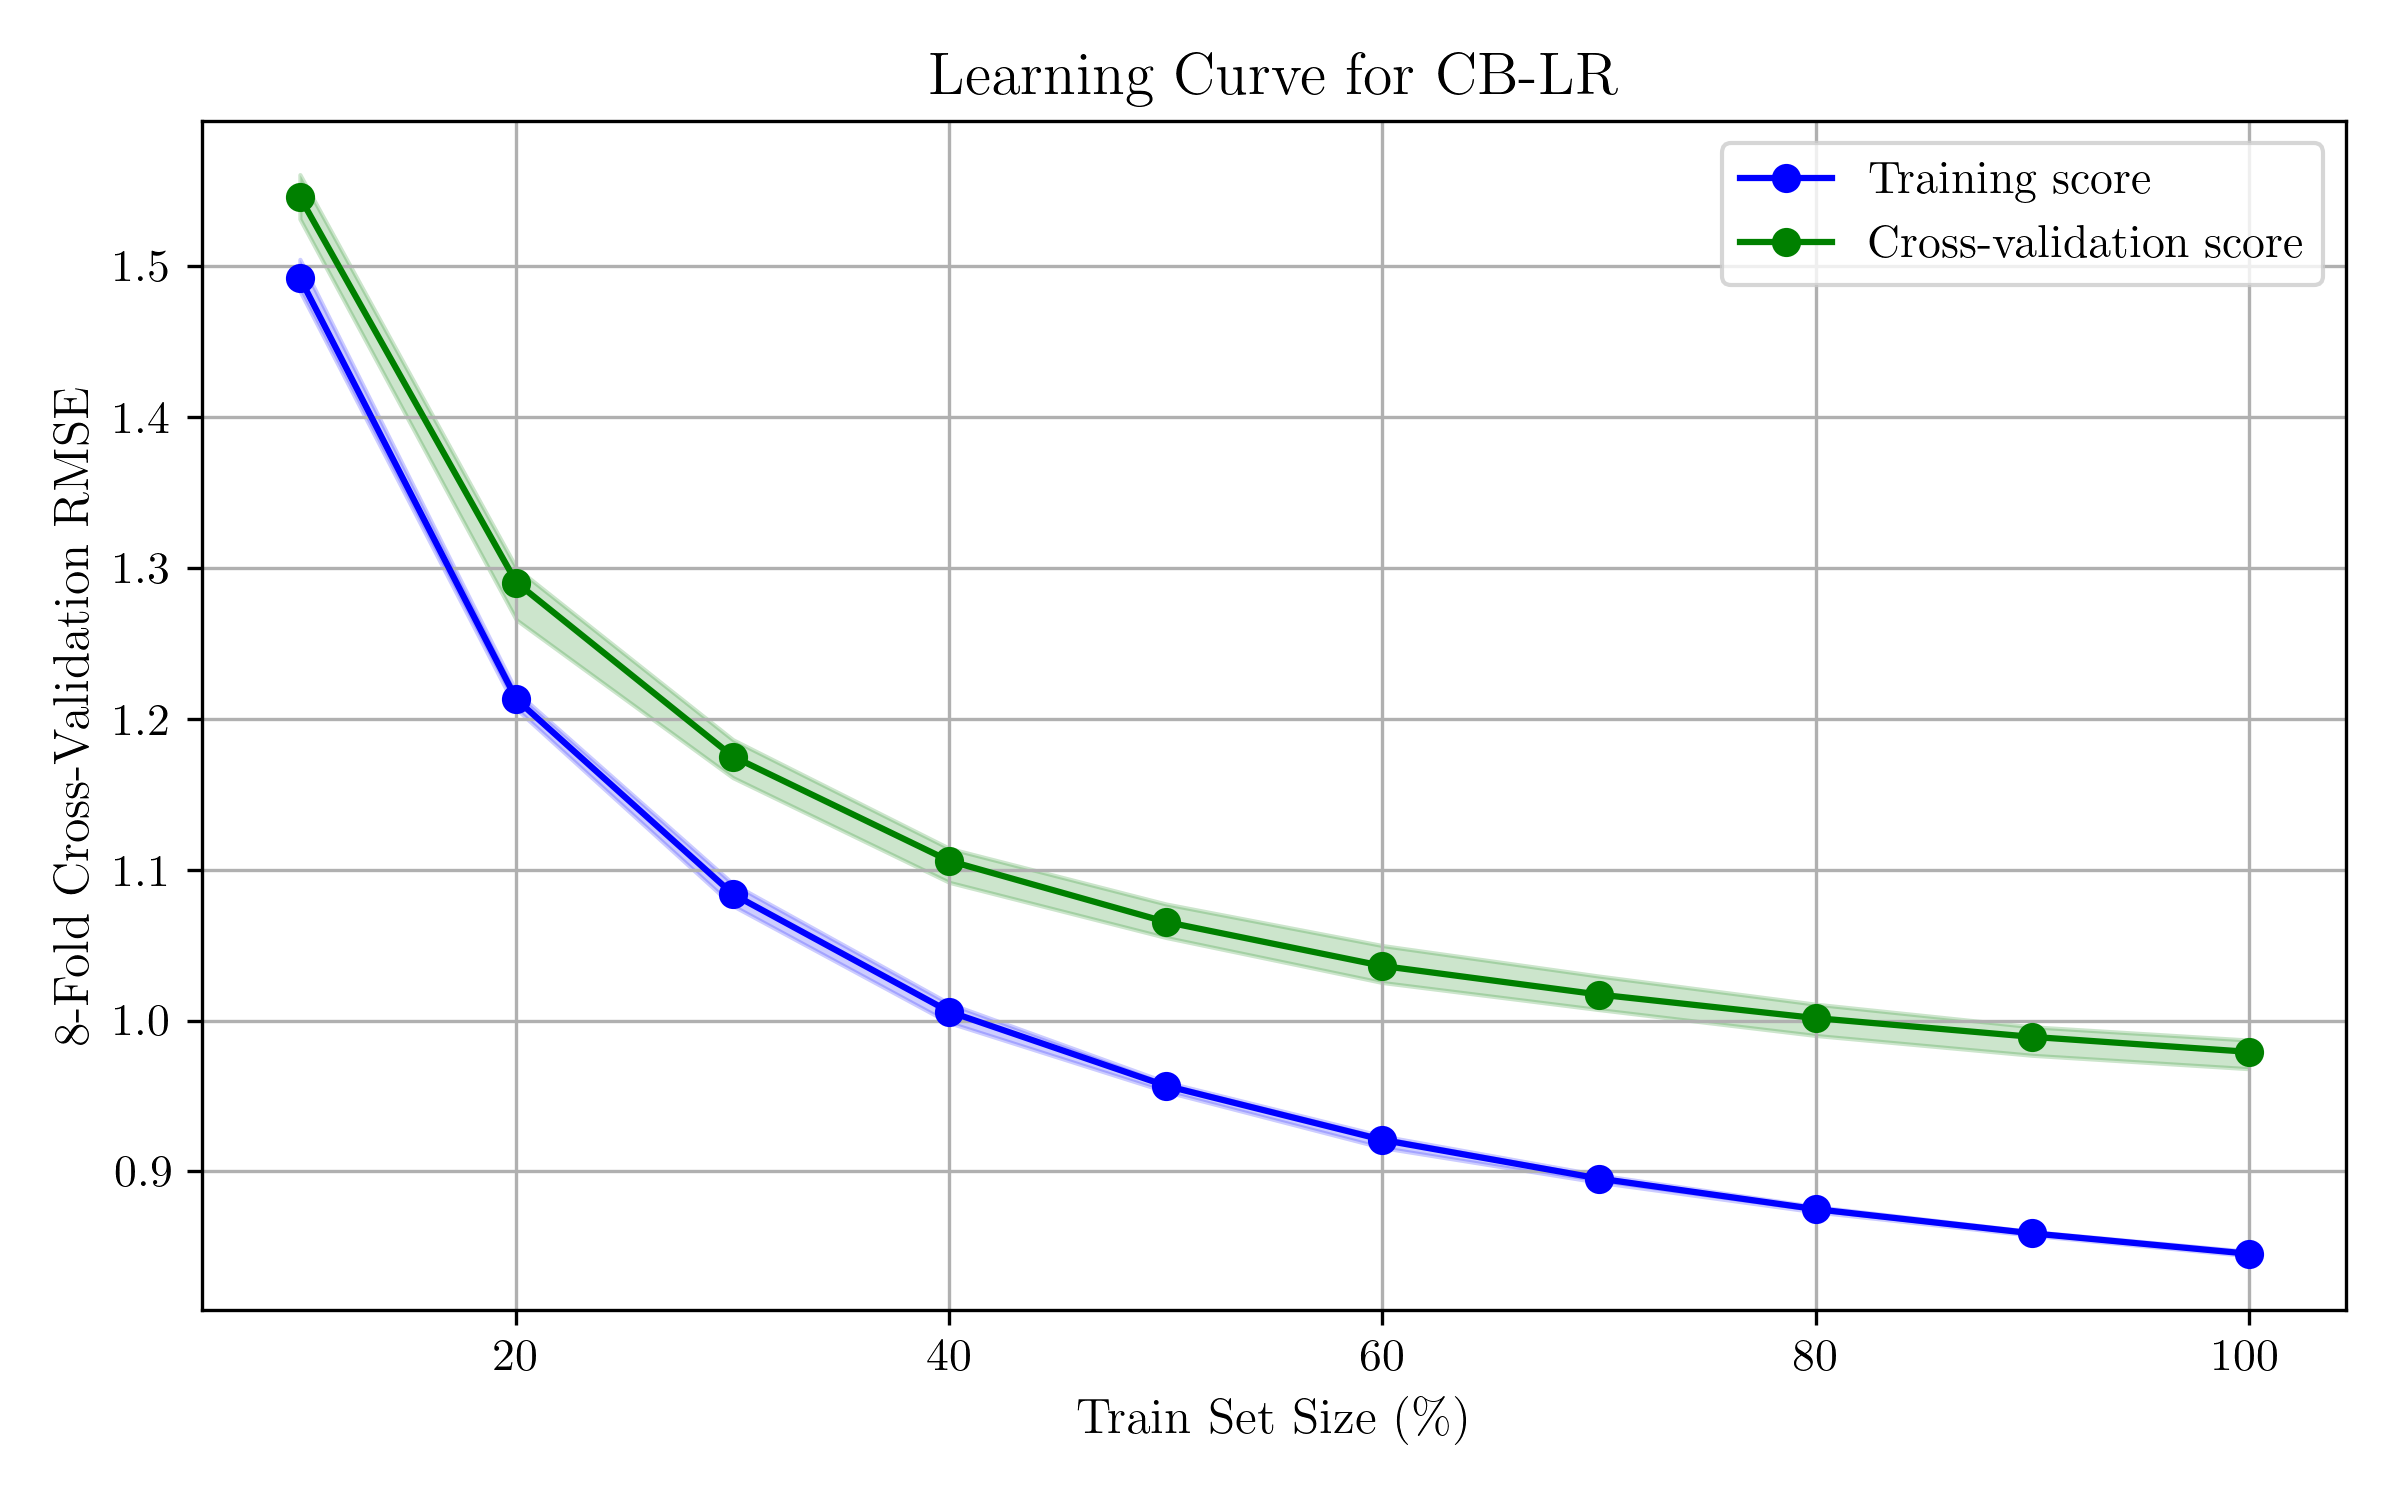
\includegraphics[width=1\linewidth]{assets/model02_learning_curve.png}
    \caption{CAPTIO CAPTION CAPTION}
    \label{fig:model02_learning_curve}
\end{figure}

e parece bastante bem, pq ambas as retas se acompanham

para alem disso tbm e importante a verificacao da convergencia do modelo, atraves da sua funcao de custo

\begin{figure}[H]
    \centering
    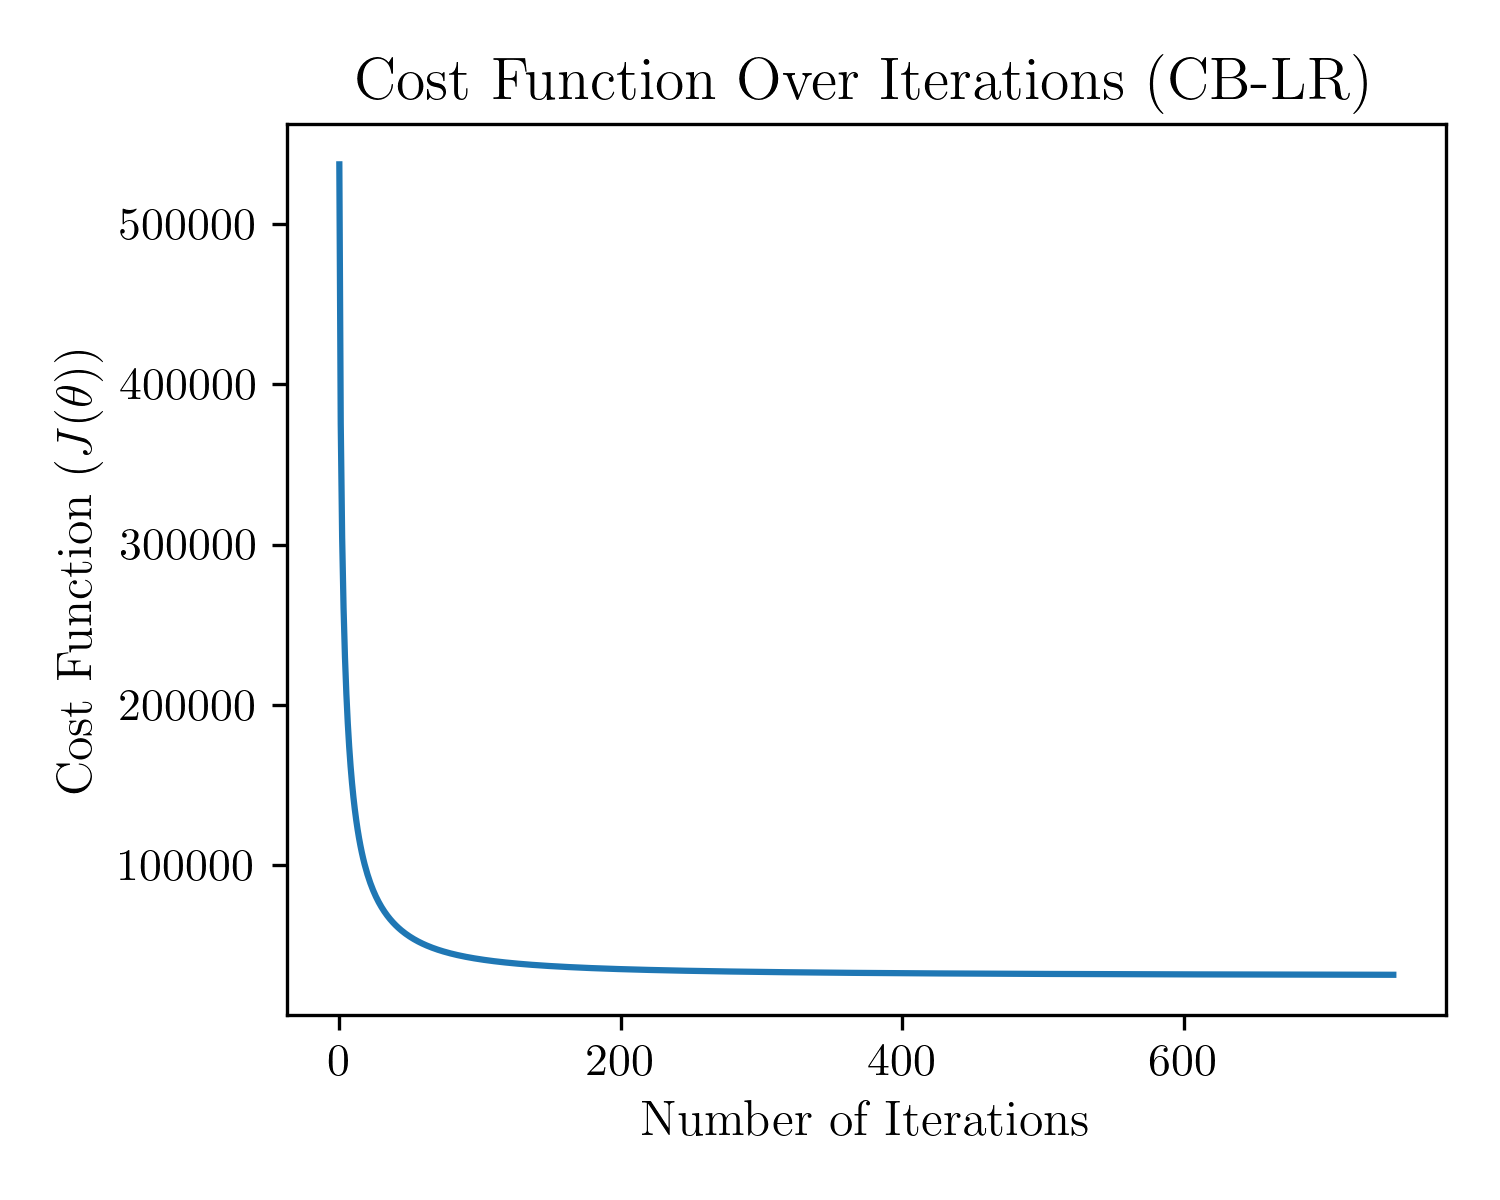
\includegraphics[width=1\linewidth]{assets/model02_cost_function.png}
    \caption{CAPTIO CAPTION CAPTION}
    \label{fig:model02_cost_function}
\end{figure}

converge e bem

atendo as medidas de erro:

\begin{table}[H]
\centering
\caption{CAPTIO CAPTION CAPTION}
\label{tab:model03_results}
\begin{tabular}{lccc}
\toprule
\textbf{Dataset} & \textbf{RMSE} & \textbf{MAE} & \textbf{Support} \\
\midrule
Train Set & 0.84859 & 0.65997 & 80668 \\
Test Set & 0.97254 & 0.74605 & 20168 \\
\bottomrule
\end{tabular}
\end{table}

medidas proximas, no signs of overfitting

\subsection{Model03 - SVD}

\begin{table}[H]
\centering
\caption{SVD model hyperparameters search space.}
\label{parametrosSVD}
\begin{tabular}{ll}
\toprule
\textbf{Hyperparameter} & \textbf{Possible Values} \\
\midrule
$n\_factors$ & \{$5,15,30,40,50$\} \\ 
$lr\_all$ & \{$0.005, 0.01, 0.05, 0.1, 1$\} \\ 
$reg\_all$ & \{$0.02,0.1,1,5,10$\} \\ 
\bottomrule
\end{tabular}
\end{table}


Number of Singular Values or Components: n\_factors

Learning rate: lr\_all

Regularization Parameters: reg\_all

Best Hyperparameters: \{'n\_factors': 50, 'lr\_all': 0.01, 'reg\_all': 0.1\}

lallla learning curve

\begin{figure}[H]
    \centering
    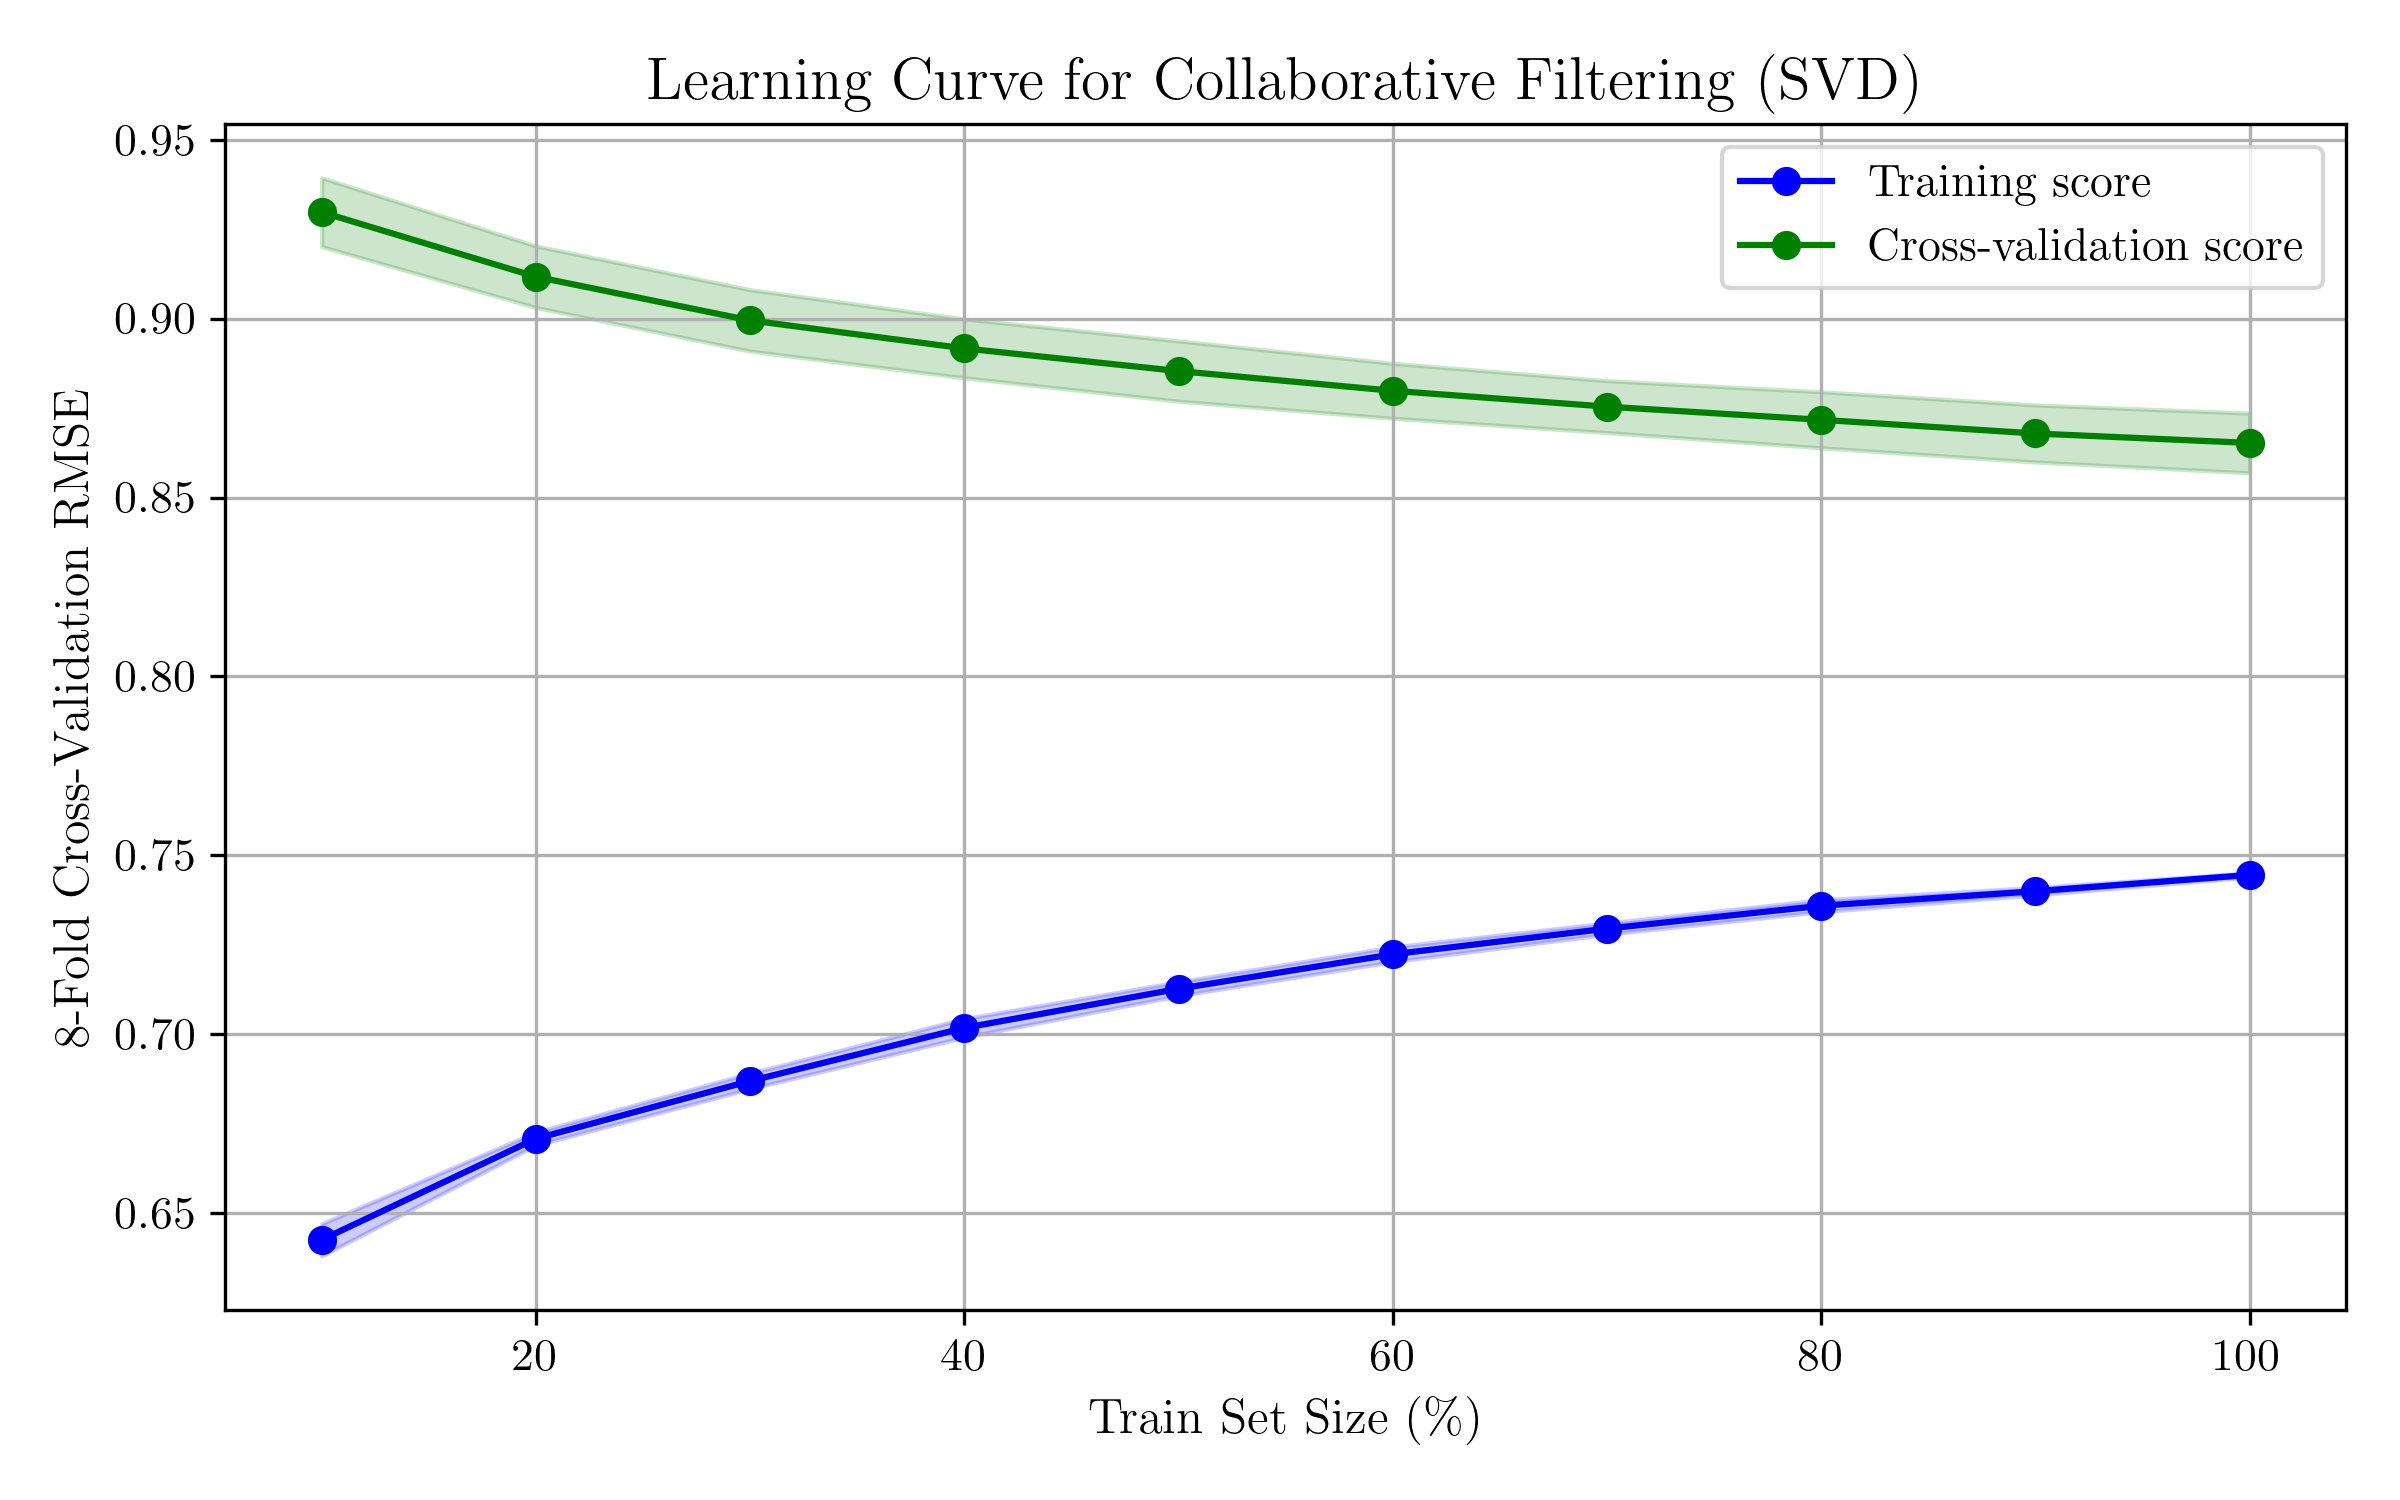
\includegraphics[width=1\linewidth]{assets/model03_learningcurve.png}
    \caption{CAPTIO CAPTION CAPTION}
    \label{fig:model03_learningcurve}
\end{figure}

lalala results meauseres

\begin{table}[H]
\centering
\caption{CAPTIO CAPTION CAPTION}
\label{tab:model03_results}
\begin{tabular}{lccc}
\toprule
\textbf{Dataset} & \textbf{RMSE} & \textbf{MAE} & \textbf{Support} \\
\midrule
Train Set & 0.75035 & 0.58313 & 80668 \\
Test Set & 0.87412 & 0.66957 & 20168 \\
\bottomrule
\end{tabular}
\end{table}


\section{Discussion} 

\subsection{Performance Metrics}

\begin{figure}[H]
    \centering
    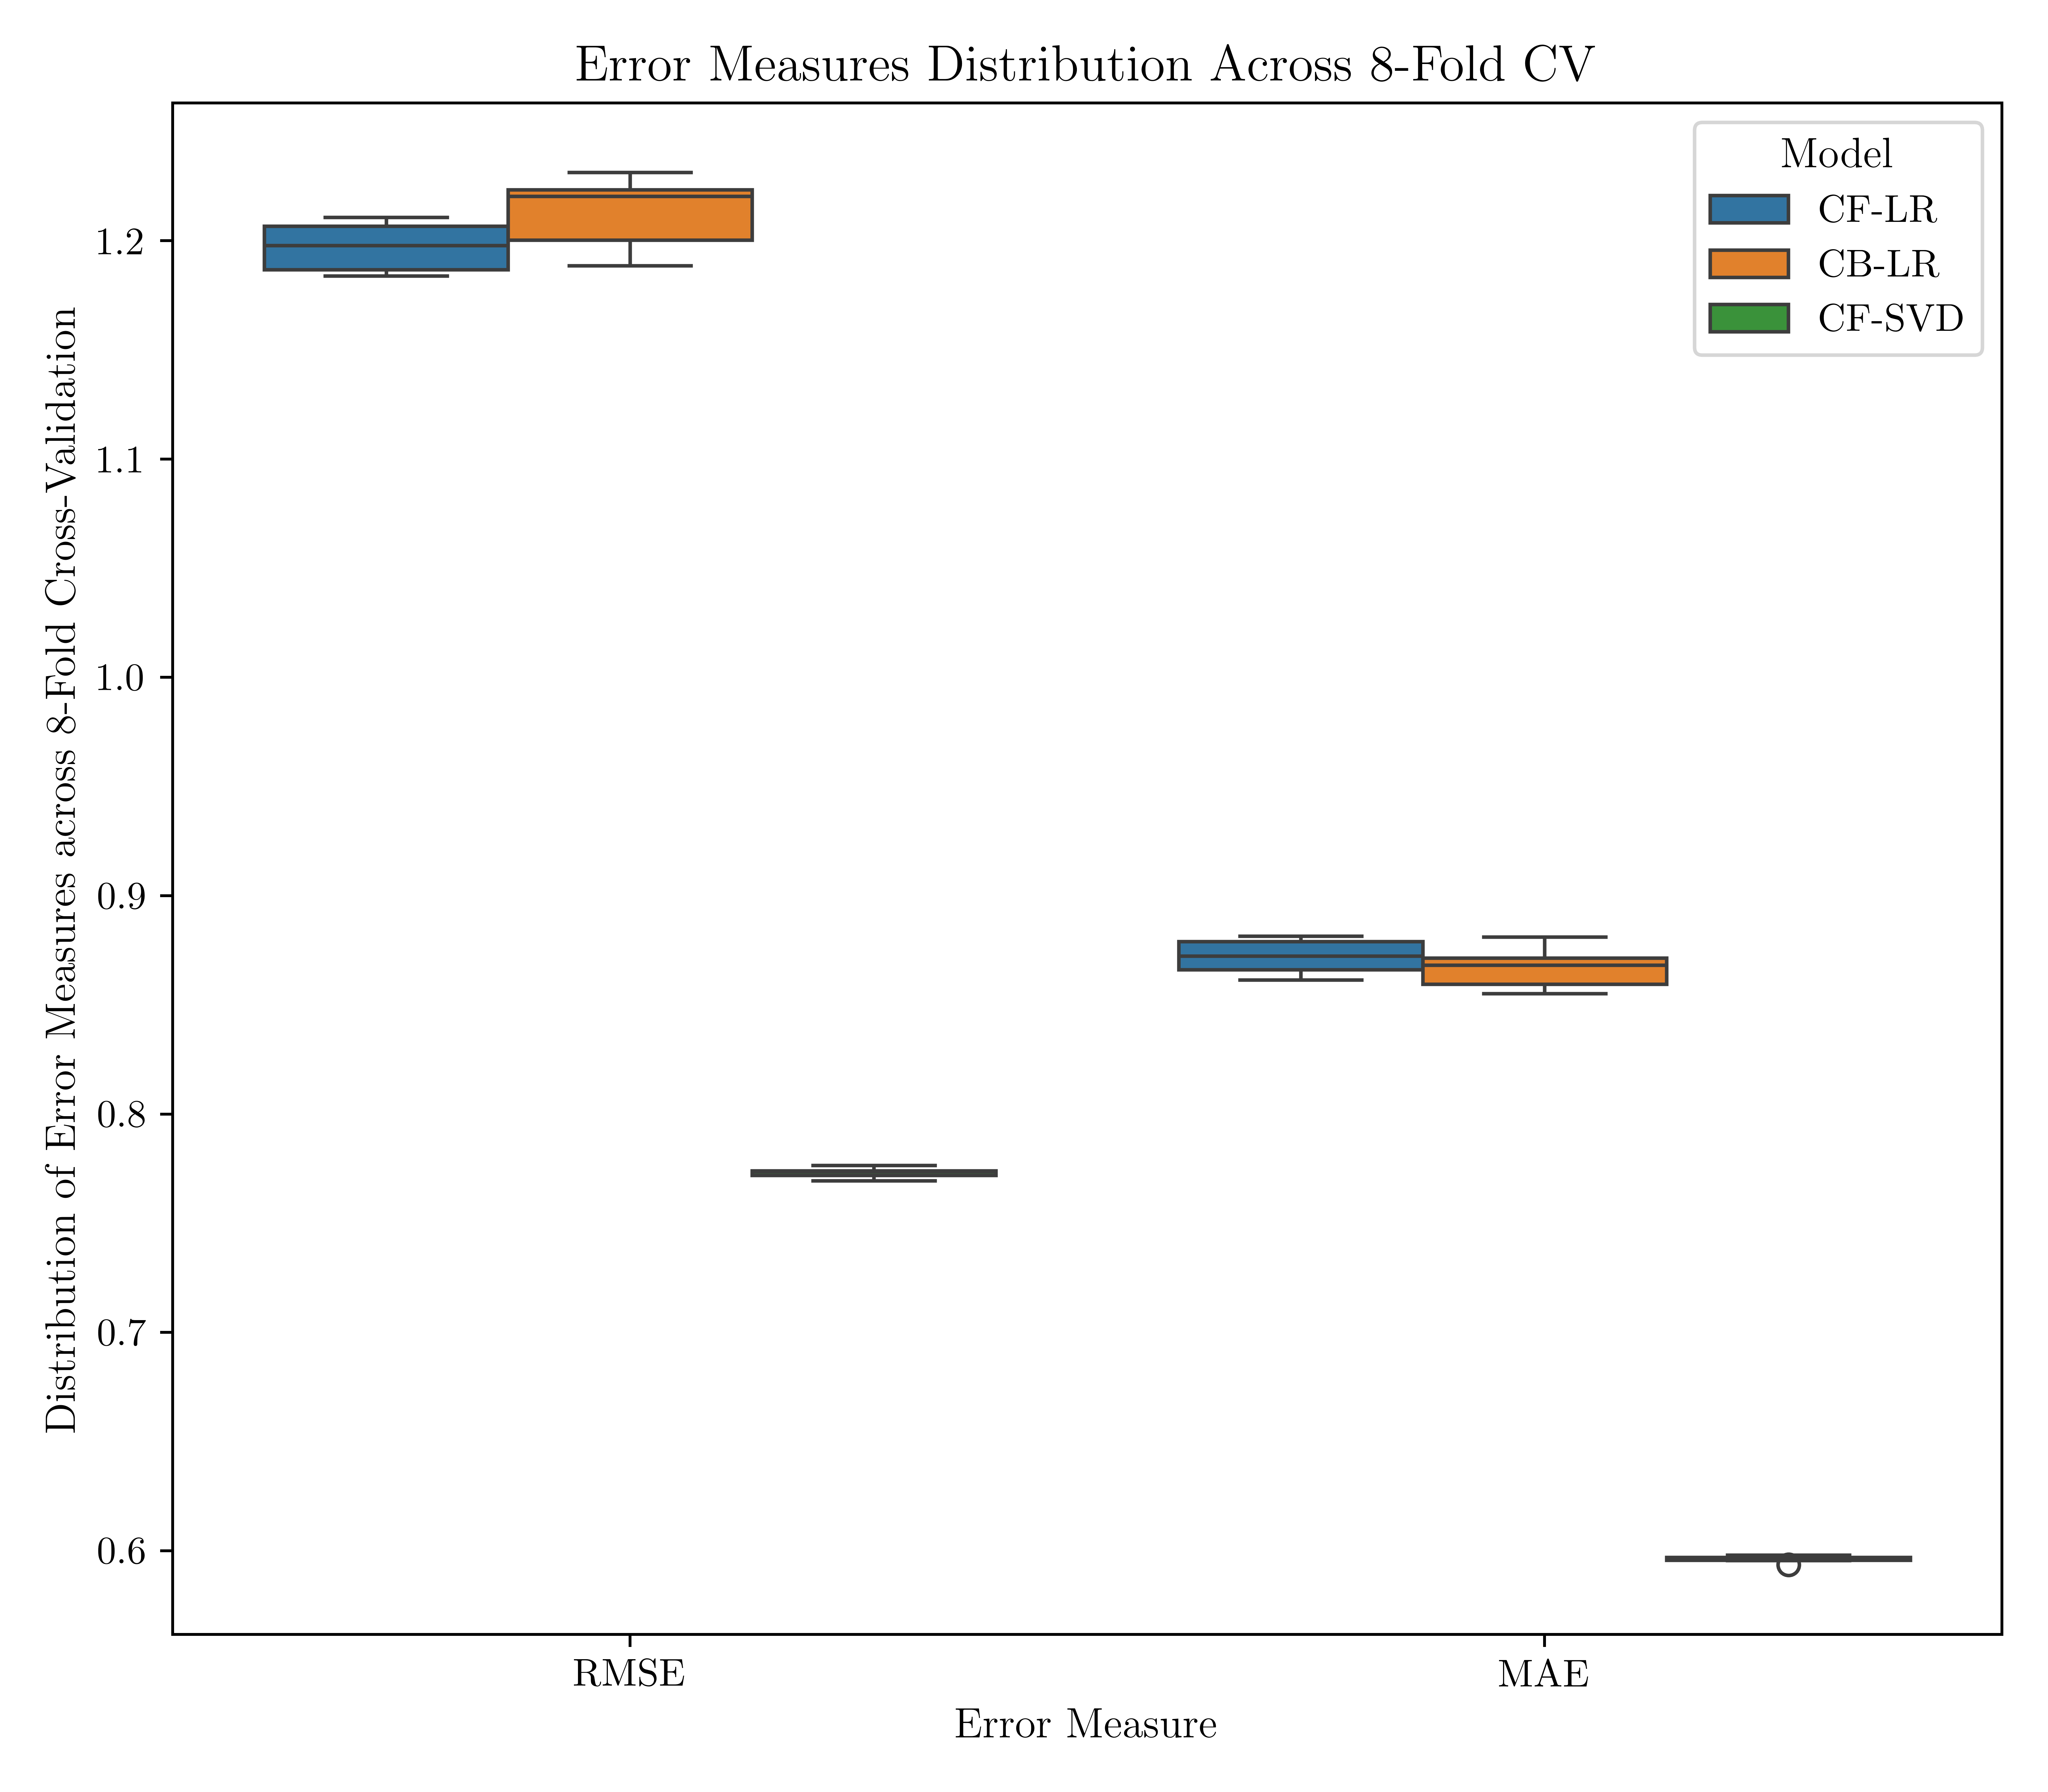
\includegraphics[width=1\linewidth]{assets/results_boxplot.png}
    \caption{caption caption caption}
    \label{fig:results_boxplot}
\end{figure}

8cv aplicado ao dataset completo: 7folds para fit, 1 fold para teste (medidas do teste apresentadas), usando os modelos otimizados


\subsection{Literature Benchmark}


\section{Conclusion}


\section*{Work Load}

Both authors contributed equally to the project.


% trigger a \newpage just before the given reference
% number - used to balance the columns on the last page
% adjust value as needed - may need to be readjusted if
% the document is modified later
%\IEEEtriggeratref{8}
% The "triggered" command can be changed if desired:
%\IEEEtriggercmd{\enlargethispage{-5in}}


\bibliographystyle{IEEEtran}
\bibliography{references}

\end{document}



